\section{PRISMA: Projection of Representations for Interpretability via Sparse Monosemantic Autoencoders}
\label{sec:05_prisma}

\epigraph{
    The purpose of abstraction is not to be vague, but to create a new semantic level in which one can be absolutely precise.
}{Edsger W. Dijkstra}

\newpage

\subsection{Fare luce nella black box degli embedding}
\label{subsec:prisma_intro}
Nel capitolo precedente abbiamo identificato i due ostacoli fondamentali che impediscono di interpretare le rappresentazioni neurali: l'opacità—non conosciamo le direzioni $\mathbf{w}_i$ lungo cui sono codificate le feature—e l'interferenza—anche conoscendole, non potremmo recuperare le intensità $a_i$ in modo pulito a causa della non-ortogonalità. Abbiamo anche delineato una via d'uscita teorica: espandere lo spazio delle rappresentazioni e imporre sparsità, così da forzare ogni feature a occupare un asse dedicato.
\begin{figure}[htbp]
    \centering
    \includegraphics[width=\textwidth]{pictures/cap5/home.png}
    \caption{Home page di PRISMA, l'applicazione sviluppata in questa tesi per la scomposizione degli embedding in feature interpretabili.}
    \label{fig:prisma_home}
\end{figure}
Questo capitolo presenta PRISMA (\textbf{P}rojection of \textbf{R}epresentations for \textbf{I}nterpretability via \textbf{S}parse \textbf{M}onosemantic \textbf{A}utoencoders), un'applicazione sviluppata in questa tesi che implementa concretamente questa strategia. Il nome non è casuale: richiama l'analogia con il prisma ottico, uno strumento che non genera luce, ma la scompone. Quando un fascio di luce bianca attraversa un prisma, ne emergono le componenti spettrali—rosso, arancione, giallo, e così via—che erano già presenti nel fascio originario, ma indistinguibili a occhio nudo. Il prisma non aggiunge informazione: la rende visibile, separando ciò che era mescolato.
\begin{figure}[htbp]
    \centering
    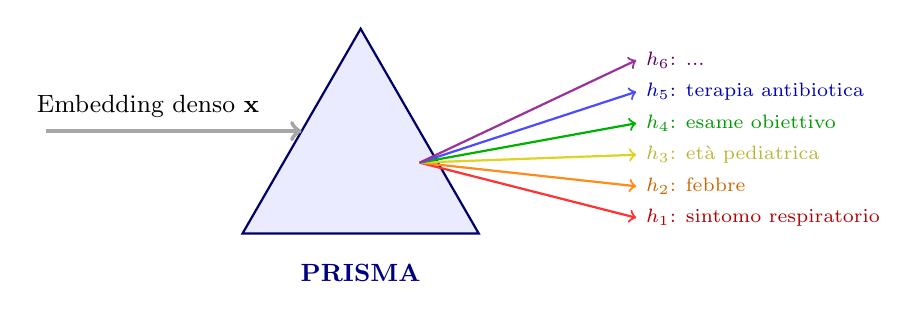
\begin{tikzpicture}[scale=1.0]
        % Prisma (triangolo)
        \coordinate (A) at (0, 0);
        \coordinate (B) at (3, 0);
        \coordinate (C) at (1.5, 2.6);
        
        \fill[blue!8] (A) -- (B) -- (C) -- cycle;
        \draw[thick, blue!40!black] (A) -- (B) -- (C) -- cycle;
        
        % Raggio incidente (bianco/grigio)
        \draw[->, ultra thick, gray!70] (-2.5, 1.3) -- (0.75, 1.3);
        \node[above, font=\small] at (-1.2, 1.35) {Embedding denso $\mathbf{x}$};
        
        % Raggi rifratti (spettro) - escono dal lato destro del prisma
        \draw[->, thick, red!80] (2.25, 0.9) -- (5, 0.2);
        \draw[->, thick, orange!90] (2.25, 0.9) -- (5, 0.6);
        \draw[->, thick, yellow!85!black] (2.25, 0.9) -- (5, 1.0);
        \draw[->, thick, green!70!black] (2.25, 0.9) -- (5, 1.4);
        \draw[->, thick, blue!70] (2.25, 0.9) -- (5, 1.8);
        \draw[->, thick, violet!80] (2.25, 0.9) -- (5, 2.2);
        
        % Etichette feature
        \node[right, font=\scriptsize, red!70!black] at (5, 0.2) {$h_1$: sintomo respiratorio};
        \node[right, font=\scriptsize, orange!80!black] at (5, 0.6) {$h_2$: febbre};
        \node[right, font=\scriptsize, yellow!70!black] at (5, 1.0) {$h_3$: età pediatrica};
        \node[right, font=\scriptsize, green!60!black] at (5, 1.4) {$h_4$: esame obiettivo};
        \node[right, font=\scriptsize, blue!70!black] at (5, 1.8) {$h_5$: terapia antibiotica};
        \node[right, font=\scriptsize, violet!70!black] at (5, 2.2) {$h_6$: ...};
        
        % Etichetta prisma
        \node[font=\small\bfseries, blue!50!black] at (1.5, -0.5) {PRISMA};
        
    \end{tikzpicture}
    \caption{L'analogia ottica di PRISMA. Come un prisma scompone la luce bianca nelle sue componenti spettrali, così PRISMA scompone un embedding denso $\mathbf{x}$ nelle sue feature semantiche costitutive $h_1, h_2, \dots, h_n$. L'informazione era già presente nell'embedding originario, ma codificata in forma opaca; PRISMA la rende esplicita e interpretabile.}
    \label{fig:prisma_analogy}
\end{figure}

PRISMA opera in modo analogo sugli embedding. Un vettore denso $\mathbf{x} \in \mathbb{R}^{768}$, prodotto da un modello come BERT, contiene informazione semantica ricchissima—ma opaca, distribuita su dimensioni che non sappiamo interpretare. PRISMA proietta questo vettore in uno spazio di dimensionalità molto maggiore ($\mathbb{R}^{n}$ con $n \gg 768$), forzando al contempo una rappresentazione sparsa: solo poche componenti $h_i$ possono essere attive per ogni input. Il risultato è una scomposizione in cui ogni componente corrisponde a una feature semantica distinta—un concetto atomico, interpretabile, che possiamo nominare.
L'analogia ha anche una seconda lettura. Il prisma, scomponendo la luce, ci permette di vedere ciò che prima era invisibile. Allo stesso modo, PRISMA fa luce sulla black box degli embedding: non aggiunge capacità predittiva al modello originario, ma rende trasparente ciò che il modello ha appreso. Se la superposition è il meccanismo con cui le reti neurali nascondono la complessità—comprimendo migliaia di concetti in poche centinaia di dimensioni—PRISMA è lo strumento che inverte questo processo, restituendoci una rappresentazione in cui possiamo finalmente leggere quali concetti sono presenti e con quale intensità.
Nel resto di questo capitolo descriveremo l'architettura tecnica che realizza questa scomposizione—lo Sparse Autoencoder—e le metodologie per interpretare automaticamente le feature estratte. Vedremo anche come le feature non siano entità isolate, ma si organizzino in strutture gerarchiche (\textit{feature families}) e come la loro granularità emerga progressivamente all'aumentare della capacità del modello (\textit{feature splitting}).
\subsection{Architettura dello Sparse Autoencoder}
\label{subsec:sae_architecture}

Lo SparseAutoencoder (SAE) è l'architettura neurale al cuore di PRISMA. Come ogni autoencoder, è composto da un encoder che mappa l'input in una rappresentazione latente e un decoder che ricostruisce l'input a partire da essa. La differenza cruciale rispetto agli autoencoder classici—trattati nel Capitolo 2—risiede in due scelte progettuali che invertono la logica tradizionale: lo spazio latente è \textit{overcomplete} anziché compresso, e le attivazioni sono forzate a essere \textit{sparse}.
\subsubsection{Panoramica dell'architettura}
\label{subsubsec:sae_overview}

Seguiamo il formalismo di O'Neill et al.~\parencite{oneill2024disentangling}. Sia $\mathbf{x} \in \mathbb{R}^d$ l'embedding di input (ad esempio, il vettore a 768 dimensioni prodotto da BERT) e $\mathbf{h} \in \mathbb{R}^n$ la rappresentazione latente, con $n > d$. L'architettura è definita da due insiemi di parametri apprendibili:
\begin{equation}
    \theta = \{W_e, \mathbf{b}_e\}, \qquad \phi = \{W_d, \mathbf{b}_d\}
\end{equation}
che parametrizzano rispettivamente l'encoder e il decoder.
L'\textbf{encoder} $f_\theta$ mappa l'input nella rappresentazione latente:
\begin{equation}
    \mathbf{h} = f_\theta(\mathbf{x}) = \sigma(W_e \mathbf{x} + \mathbf{b}_e)
    \label{eq:sae_encoder}
\end{equation}
dove $W_e \in \mathbb{R}^{n \times d}$ è la matrice dei pesi, $\mathbf{b}_e \in \mathbb{R}^n$ è il vettore di bias, e $\sigma(\cdot)$ è una funzione di attivazione non lineare (tipicamente ReLU).
Il \textbf{decoder} $g_\phi$ ricostruisce l'input dalla rappresentazione latente:
\begin{equation}
    \hat{\mathbf{x}} = g_\phi(\mathbf{h}) = W_d \mathbf{h} + \mathbf{b}_d
    \label{eq:sae_decoder}
\end{equation}
dove $W_d \in \mathbb{R}^{d \times n}$ è la matrice dei pesi e $\mathbf{b}_d \in \mathbb{R}^d$ è il vettore di bias.
La Figura~\ref{fig:sae_architecture} illustra il flusso dei dati attraverso l'architettura. Si noti immediatamente l'asimmetria nelle dimensioni: l'input $\mathbf{x}$ ha $d$ componenti, mentre la rappresentazione latente $\mathbf{h}$ ne ha $n \gg d$. Questa espansione—l'opposto della compressione tipica degli autoencoder—è la prima chiave per ottenere il disentanglement. La seconda chiave, visibile nei pochi cerchi verdi tra i molti grigi, è la sparsità: per ogni input, solo una piccola frazione delle $n$ componenti di $\mathbf{h}$ è diversa da zero.
\begin{figure}[htbp]
    \centering
    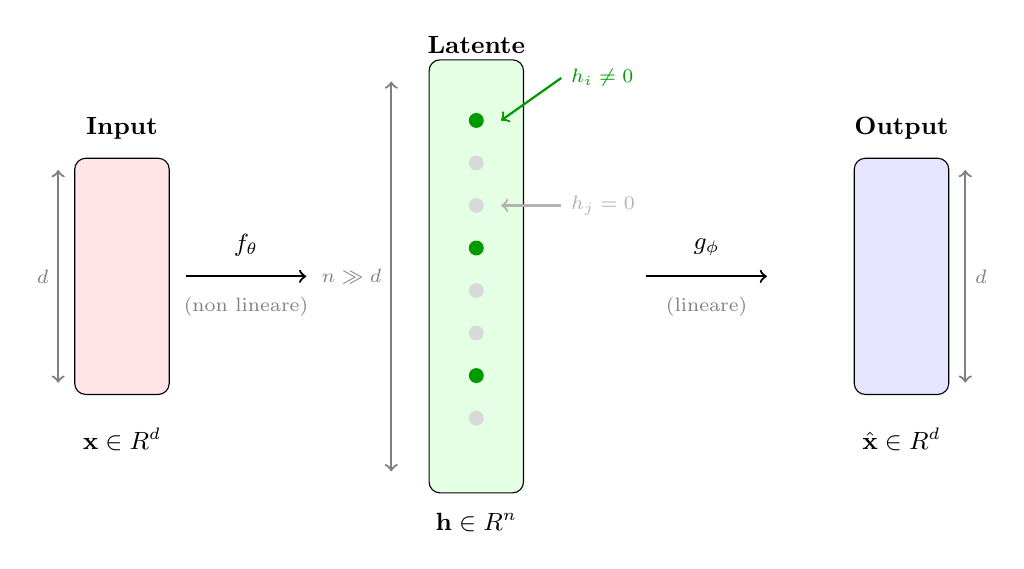
\begin{tikzpicture}[scale=0.9]
        % Input
        \node[draw, rectangle, minimum width=1.2cm, minimum height=3cm, fill=red!10, rounded corners] (input) at (0, 0) {};
        \node[below, font=\small] at (0, -2.0) {$\mathbf{x} \in \mathbb{R}^d$};
        \node[above, font=\small\bfseries] at (0, 1.8) {Input};
        
        % Encoder arrow
        \draw[->, thick] (0.9, 0) -- (2.6, 0);
        \node[above, font=\small] at (1.75, 0.15) {$f_\theta$};
        \node[below, font=\scriptsize, gray] at (1.75, -0.15) {(non lineare)};
        
        % Latent space (overcomplete)
        \node[draw, rectangle, minimum width=1.2cm, minimum height=5.5cm, fill=green!10, rounded corners] (latent) at (5, 0) {};
        \node[below, font=\small] at (5, -3.2) {$\mathbf{h} \in \mathbb{R}^n$};
        \node[above, font=\small\bfseries] at (5, 3.0) {Latente};
        
        % Sparse activations (dots)
        \fill[green!60!black] (5, 2.2) circle (3pt);
        \fill[gray!30] (5, 1.6) circle (3pt);
        \fill[gray!30] (5, 1.0) circle (3pt);
        \fill[green!60!black] (5, 0.4) circle (3pt);
        \fill[gray!30] (5, -0.2) circle (3pt);
        \fill[gray!30] (5, -0.8) circle (3pt);
        \fill[green!60!black] (5, -1.4) circle (3pt);
        \fill[gray!30] (5, -2.0) circle (3pt);
        
        % Annotation for sparsity
        \draw[<-, thick, green!60!black] (5.35, 2.2) -- (6.2, 2.8);
        \node[right, font=\scriptsize, green!60!black, align=left] at (6.2, 2.8) {$h_i \neq 0$};
        
        \draw[<-, thick, gray!60] (5.35, 1.0) -- (6.2, 1.0);
        \node[right, font=\scriptsize, gray!60, align=left] at (6.2, 1.0) {$h_j = 0$};
        
        % Decoder arrow
        \draw[->, thick] (7.4, 0) -- (9.1, 0);
        \node[above, font=\small] at (8.25, 0.15) {$g_\phi$};
        \node[below, font=\scriptsize, gray] at (8.25, -0.15) {(lineare)};
        
        % Output
        \node[draw, rectangle, minimum width=1.2cm, minimum height=3cm, fill=blue!10, rounded corners] (output) at (11, 0) {};
        \node[below, font=\small] at (11, -2.0) {$\hat{\mathbf{x}} \in \mathbb{R}^d$};
        \node[above, font=\small\bfseries] at (11, 1.8) {Output};
        
        % Dimension annotations
        \draw[<->, thick, gray] (-0.9, -1.5) -- (-0.9, 1.5);
        \node[left, font=\scriptsize, gray] at (-0.9, 0) {$d$};
        
        \draw[<->, thick, gray] (3.8, -2.75) -- (3.8, 2.75);
        \node[left, font=\scriptsize, gray] at (3.8, 0) {$n \gg d$};
        
        \draw[<->, thick, gray] (11.9, -1.5) -- (11.9, 1.5);
        \node[right, font=\scriptsize, gray] at (11.9, 0) {$d$};
        
    \end{tikzpicture}
    \caption{Architettura dello Sparse Autoencoder. L'encoder $f_\theta$ (non lineare) mappa l'input $\mathbf{x}$ in uno spazio latente \textit{overcomplete} di dimensione $n \gg d$. La sparsità forza solo poche componenti di $\mathbf{h}$ (cerchi verdi) ad essere attive, mentre le altre (cerchi grigi) restano nulle. Il decoder $g_\phi$ (lineare) ricostruisce l'input come combinazione delle sole direzioni attive.}
    \label{fig:sae_architecture}
\end{figure}
Un'asimmetria meno evidente, ma altrettanto importante, riguarda la natura delle due trasformazioni: l'encoder è non lineare (Equazione~\ref{eq:sae_encoder}), mentre il decoder è lineare (Equazione~\ref{eq:sae_decoder}). Questa scelta non è arbitraria: come vedremo nelle prossime sezioni, è precisamente la linearità del decoder a garantire che le feature estratte siano interpretabili come direzioni nello spazio degli embedding—la condizione necessaria per ottenere il disentanglement discusso nel Capitolo~\ref{sec:04_disentangling_dense_embeddings_with_sparse_autoencoders}.
subsubsection{L'encoder: una proiezione non lineare}
\label{subsubsec:sae_encoder}

L'encoder ha il compito di analizzare l'embedding in ingresso e determinare quali feature sono presenti e con quale intensità. Riprendendo l'Equazione~\ref{eq:sae_encoder}:
\begin{equation}
    \mathbf{h} = f_\theta(\mathbf{x}) = \sigma(W_e \mathbf{x} + \mathbf{b}_e)
\end{equation}
questa trasformazione si compone di due passaggi: una proiezione lineare $W_e \mathbf{x} + \mathbf{b}_e$ seguita da una non linearità $\sigma(\cdot)$.
La matrice $W_e \in \mathbb{R}^{n \times d}$ ha $n$ righe, una per ogni componente dello spazio latente. Indichiamo con $\mathbf{e}_i^T$ la $i$-esima riga: è un vettore in $\mathbb{R}^d$ che vive nello stesso spazio dell'input $\mathbf{x}$. La proiezione lineare calcola, per ogni feature $i$, un punteggio grezzo:
\begin{equation}
    z_i = \mathbf{e}_i^T \mathbf{x} + b_{e,i}
\end{equation}
Questo punteggio misura quanto l'input $\mathbf{x}$ sia allineato con la direzione $\mathbf{e}_i$: se i due vettori puntano in direzioni simili, il prodotto scalare sarà elevato; se puntano in direzioni opposte, sarà negativo.
La non linearità $\sigma(\cdot)$—tipicamente la funzione ReLU—trasforma i punteggi grezzi nelle attivazioni finali:
\begin{equation}
    h_i = \sigma(z_i) = \max(0, z_i)
\end{equation}
La scelta della ReLU serve a due scopi. Il primo è garantire attivazioni non negative: una feature è ``presente'' con una certa intensità positiva, oppure è ``assente'' (attivazione nulla). Non avrebbe senso, dal punto di vista interpretativo, che una feature fosse presente con intensità negativa. Il secondo scopo è indurre sparsità naturale: la ReLU azzera tutte le pre-attivazioni negative, contribuendo alla sparsità della rappresentazione anche prima di applicare vincoli espliciti come il Top-K che vedremo nella Sezione~\ref{subsec:loss_function}.
\begin{figure}[htbp]
    \centering
    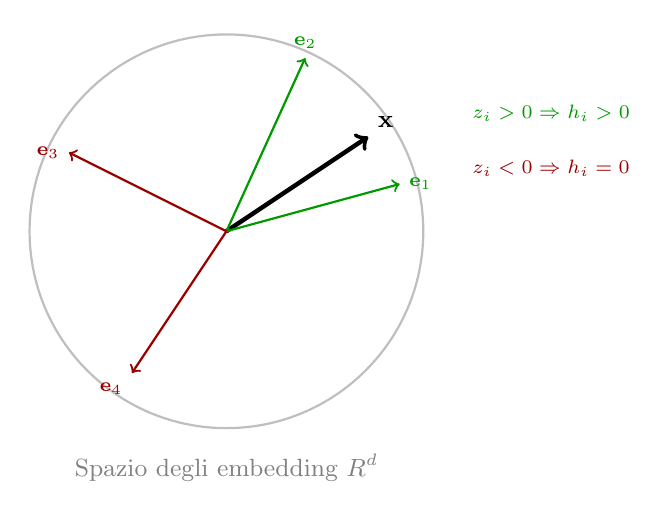
\begin{tikzpicture}[scale=1.0]
        % Spazio embedding (cerchio)
        \draw[thick, gray!50] (0,0) circle (2.5cm);
        \node[font=\small, gray] at (0, -3.0) {Spazio degli embedding $\mathbb{R}^d$};
        
        % Vettore input x
        \draw[->, ultra thick, black] (0,0) -- (1.8, 1.2);
        \node[above right, font=\small\bfseries] at (1.8, 1.2) {$\mathbf{x}$};
        
        % Direzioni di rilevamento encoder
        \draw[->, thick, green!60!black] (0,0) -- (2.2, 0.6);
        \node[right, font=\scriptsize, green!60!black] at (2.2, 0.6) {$\mathbf{e}_1$};
        
        \draw[->, thick, green!60!black] (0,0) -- (1.0, 2.2);
        \node[above, font=\scriptsize, green!60!black] at (1.0, 2.2) {$\mathbf{e}_2$};
        
        \draw[->, thick, red!60!black] (0,0) -- (-2.0, 1.0);
        \node[left, font=\scriptsize, red!60!black] at (-2.0, 1.0) {$\mathbf{e}_3$};
        
        \draw[->, thick, red!60!black] (0,0) -- (-1.2, -1.8);
        \node[below left, font=\scriptsize, red!60!black] at (-1.2, -1.8) {$\mathbf{e}_4$};
        
        % Legenda
        \node[right, font=\scriptsize, green!60!black] at (3.0, 1.5) {$z_i > 0 \Rightarrow h_i > 0$};
        \node[right, font=\scriptsize, red!60!black] at (3.0, 0.8) {$z_i < 0 \Rightarrow h_i = 0$};
        
    \end{tikzpicture}
    \caption{L'encoder come rilevatore di feature. L'input $\mathbf{x}$ viene proiettato sulle direzioni $\mathbf{e}_i$ (righe di $W_e$). Le direzioni sufficientemente allineate con $\mathbf{x}$ (in verde) producono pre-attivazioni positive $z_i > 0$, che la ReLU preserva; quelle non allineate (in rosso) producono $z_i < 0$ e vengono azzerate.}
    \label{fig:encoder_detection}
\end{figure}

È importante chiarire il ruolo di questi vettori $\mathbf{e}_i$. Essi non coincidono con le direzioni $\mathbf{w}_i$ introdotte nel Capitolo~\ref{sec:04_disentangling_dense_embeddings_with_sparse_autoencoders}: le $\mathbf{w}_i$ sono le direzioni lungo cui le feature sono \textit{codificate} nello spazio degli embedding, e corrispondono—come vedremo—alle colonne della matrice del decoder $W_d$. Le $\mathbf{e}_i$, invece, sono direzioni ausiliarie che l'encoder utilizza per \textit{rilevare} le feature nell'input. In uno scenario ideale con feature perfettamente ortogonali, le due coinciderebbero: per rilevare una feature basterebbe proiettare lungo la sua stessa direzione. Ma nella superposition le $\mathbf{w}_i$ non sono ortogonali, e proiettare direttamente lungo di esse causerebbe l'interferenza descritta nel capitolo precedente. L'encoder impara quindi direzioni $\mathbf{e}_i \neq \mathbf{w}_i$ che compensano questa sovrapposizione.
Dal punto di vista dell'interpretabilità, le $\mathbf{e}_i$ non hanno un significato semantico diretto: sono un meccanismo interno che serve all'encoder per svolgere il suo compito. Ciò che ci interessa—e che costituisce il vero output interpretabile del SAE—sono le attivazioni $h_i$ e le direzioni $\mathbf{w}_i$ del decoder. La corrispondenza è uno-a-uno: per ogni $i \in \{1, \dots, n\}$, il vettore $\mathbf{e}_i$ rileva la feature $i$ producendo l'attivazione $h_i$, che a sua volta pesa la direzione $\mathbf{w}_i$ nella ricostruzione. Ma mentre $\mathbf{e}_i$ è un dettaglio implementativo, $\mathbf{w}_i$ rappresenta la feature stessa nello spazio semantico.
La non linearità dell'encoder è dunque essenziale: permette di implementare una logica di rilevamento sofisticata in presenza di sovrapposizione. Il decoder, come vedremo, ha un compito diverso—ricostruire l'input come combinazione di feature—e per quel compito la linearità non è solo possibile, ma necessaria.

\subsubsection{Lo spazio latente overcomplete}
\label{subsubsec:sae_overcomplete}
Nel Capitolo~\ref{sec:04_disentangling_dense_embeddings_with_sparse_autoencoders} abbiamo identificato il paradosso della capacità: un modello come BERT rappresenta decine di migliaia di concetti con soli 768 neuroni. La superposition risolve questo problema comprimendo le feature come direzioni oblique, ma al costo dell'opacità e dell'interferenza. Se vogliamo invertire questo processo—ottenere una rappresentazione in cui ogni feature abbia un asse dedicato—servono più dimensioni di quelle originarie.
Questa è l'intuizione alla base dello spazio latente \textit{overcomplete}. A differenza degli autoencoder classici, che comprimono l'input in un bottleneck di dimensionalità inferiore ($n < d$), lo Sparse Autoencoder espande la rappresentazione in uno spazio più grande:
\begin{equation}
    n > d
\end{equation}
dove $d$ è la dimensionalità dell'embedding originale e $n$ è la dimensionalità dello spazio latente.
Il rapporto tra queste due quantità è detto \textit{expansion factor}:
\begin{equation}
    \rho = \frac{n}{d}
\end{equation}
e assume tipicamente valori compresi tra 2 e 9~\parencite{oneill2024disentangling}. Un expansion factor $\rho = 4$, ad esempio, significa che lo spazio latente ha quattro volte le dimensioni dell'input: per un embedding BERT a 768 dimensioni, lo spazio latente avrebbe $n = 3072$ componenti.
\begin{figure}[htbp]
    \centering
    \begin{tikzpicture}[scale=1, transform shape, node distance=1cm]
        % Nodes
        \node[draw, rectangle, minimum height=3cm, minimum width=0.5cm, fill=gray!20] (input) at (0,0) {$\mathbf{x} \in \mathbb{R}^{d}$};
        \node[draw, trapezium, trapezium angle=70, shape border rotate=270, minimum height=1.5cm, fill=orange!15] (enc) at (2.5,0) {Encoder};
        \node[draw, rectangle, minimum height=1.2cm, minimum width=0.5cm, fill=orange!30] (latent) at (5,0) {$\mathbf{z} \in \mathbb{R}^{m}$};
        \node at (5, -1.5) {\footnotesize $m < d$};
        \node[draw, trapezium, trapezium angle=70, shape border rotate=90, minimum height=1.5cm, fill=orange!15] (dec) at (7.5,0) {Decoder};
        \node[draw, rectangle, minimum height=3cm, minimum width=0.5cm, fill=gray!20] (output) at (10,0) {$\hat{\mathbf{x}} \in \mathbb{R}^{d}$};
        % Arrows
        \draw[->, thick] (input) -- (enc);
        \draw[->, thick] (enc) -- (latent);
        \draw[->, thick] (latent) -- (dec);
        \draw[->, thick] (dec) -- (output);
    \end{tikzpicture}
    \caption{Autoencoder classico: il bottleneck forza la compressione informativa ($m < d$).}
    \label{fig:ae_classico}
\end{figure}

\begin{figure}[htbp]
    \centering
    \begin{tikzpicture}[scale=1, transform shape, node distance=1cm]
        % Nodes
        \node[draw, rectangle, minimum height=2cm, minimum width=0.5cm, fill=gray!20] (input) at (0,0) {$\mathbf{x} \in \mathbb{R}^{d}$};
        
        % Trapezium for Expansion
        \node[draw, trapezium, trapezium angle=70, shape border rotate=90, minimum height=1.5cm, fill=green!15] (enc) at (2.5,0) {Encoder};
        
        % Sparse Latent
        \node[draw, rectangle, minimum height=4cm, minimum width=0.5cm, fill=green!30, label=above:spazio latente $\mathbf{h}$] (latent) at (5,0) {$\mathbf{h} \in \mathbb{R}^{n}$};
        \node at (5, -2.8) {\footnotesize $n > d$};
        
        % Trapezium for Compression
        \node[draw, trapezium, trapezium angle=70, shape border rotate=270, minimum height=1.5cm, fill=green!15] (dec) at (7.5,0) {Decoder};
        
        \node[draw, rectangle, minimum height=2cm, minimum width=0.5cm, fill=gray!20] (output) at (10,0) {$\hat{\mathbf{x}} \in \mathbb{R}^{d}$};
        % Arrows
        \draw[->, thick] (input) -- (enc);
        \draw[->, thick] (enc) -- (latent);
        \draw[->, thick] (latent) -- (dec);
        \draw[->, thick] (dec) -- (output);
    \end{tikzpicture}
    \caption{Sparse Autoencoder: lo spazio latente è overcomplete ($n > d$), con abbastanza dimensioni affinché ogni feature possa avere un asse dedicato.}
    \label{fig:sae_overcomplete}
\end{figure}
La scelta di $\rho$ riflette un compromesso. Valori troppo bassi potrebbero non fornire abbastanza dimensioni per rappresentare tutte le feature del modello originario: se BERT codifica 50.000 concetti in 768 dimensioni, un expansion factor $\rho = 2$ fornirebbe solo 1.536 assi—ancora insufficienti per il disentanglement completo. Valori troppo alti, d'altra parte, aumentano il costo computazionale e il rischio di overfitting: con troppe dimensioni disponibili, il modello potrebbe apprendere feature spurie o ridondanti.
Nella pratica, la scelta dell'expansion factor dipende dal dominio e dalla granularità desiderata. O'Neill et al.~\parencite{oneill2024disentangling} osservano che, per embedding di articoli scientifici, valori di $\rho$ tra 2 e 6 producono feature interpretabili con un buon compromesso tra capacità e qualità. Expansion factor maggiori tendono a produrre feature più specifiche e granulari—un fenomeno che esploreremo nella Sezione~\ref{subsec:feature_splitting} sotto il nome di \textit{feature splitting}.
È importante sottolineare che l'overcompletezza, da sola, non garantisce il disentanglement. Uno spazio con $n > d$ dimensioni offre la \textit{possibilità} che ogni feature abbia un asse dedicato, ma nulla impedisce al modello di utilizzare questo spazio in modo ridondante o non interpretabile. È il vincolo di sparsità—che vedremo nella Sezione~\ref{subsec:loss_function}—a forzare il modello a sfruttare l'overcompletezza nel modo desiderato: poche attivazioni per input, ciascuna corrispondente a una feature distinta.

\subsubsection{La linearità del decoder: la chiave del disentanglement}
\label{subsubsec:sae_decoder_linearity}
Abbiamo visto che l'encoder è una funzione non lineare: la ReLU introduce una soglia che azzera le attivazioni negative, permettendo di rilevare le feature in modo selettivo. Il decoder, al contrario, è una trasformazione puramente lineare. Riprendendo l'Equazione~\ref{eq:sae_decoder}:
\begin{equation}
    \hat{\mathbf{x}} = g_\phi(\mathbf{h}) = W_d \mathbf{h} + \mathbf{b}_d
\end{equation}
Questa asimmetria non è un dettaglio implementativo: è la scelta architetturale che rende possibile il disentanglement. Per capire perché, espandiamo il prodotto matrice-vettore $W_d \mathbf{h}$. La matrice $W_d \in \mathbb{R}^{d \times n}$ ha $n$ colonne; indichiamo la $i$-esima colonna con $\mathbf{w}_i \in \mathbb{R}^d$. Il vettore $\mathbf{h} \in \mathbb{R}^n$ ha $n$ componenti $h_1, h_2, \dots, h_n$. Il prodotto può essere scritto come:
\begin{equation}
    W_d \mathbf{h} = \sum_{i=1}^{n} h_i \cdot \mathbf{w}_i
    \label{eq:decoder_linear_combination}
\end{equation}
La ricostruzione completa diventa quindi:
\begin{equation}
    \hat{\mathbf{x}} = \sum_{i=1}^{n} h_i \cdot \mathbf{w}_i + \mathbf{b}_d
    \label{eq:reconstruction_explicit}
\end{equation}
Questa equazione è il cuore dell'interpretabilità dello Sparse Autoencoder. La ricostruzione $\hat{\mathbf{x}}$ è una \textit{combinazione lineare} dei vettori $\mathbf{w}_i$, pesata dalle attivazioni $h_i$. Ogni vettore $\mathbf{w}_i$ rappresenta il contributo che la feature $i$ apporta alla ricostruzione quando è attiva con intensità unitaria. L'attivazione $h_i$ modula questo contributo: se $h_i = 0$ la feature non contribuisce; se $h_i > 0$, il vettore $\mathbf{w}_i$ viene sommato alla ricostruzione con peso proporzionale all'intensità della feature.
I vettori $\mathbf{w}_i$ sono esattamente le direzioni delle feature di cui abbiamo parlato nel Capitolo~\ref{sec:04_disentangling_dense_embeddings_with_sparse_autoencoders}. Là avevamo scritto l'embedding come combinazione di direzioni sconosciute:
\begin{equation}
    \mathbf{x} = \sum_i a_i \, \mathbf{w}_i
\end{equation}
lamentando di non conoscere né le direzioni $\mathbf{w}_i$ né le intensità $a_i$. Lo Sparse Autoencoder risolve entrambi i problemi: le direzioni $\mathbf{w}_i$ sono le colonne della matrice $W_d$, apprese durante l'addestramento e quindi note; le intensità $a_i$ corrispondono alle attivazioni $h_i$, calcolate dall'encoder per ogni input.
\begin{notebox}
\textbf{La chiave del disentanglement}\\
Nel Capitolo~\ref{sec:04_disentangling_dense_embeddings_with_sparse_autoencoders} abbiamo identificato due problemi della superposition:
\begin{enumerate}
    \item \textbf{Opacità}: non conosciamo le direzioni $\mathbf{w}_i$ delle feature
    \item \textbf{Interferenza}: non possiamo recuperare le intensità $a_i$ a causa della non-ortogonalità
\end{enumerate}
Lo Sparse Autoencoder affronta entrambi:
\begin{enumerate}
    \item Le direzioni $\mathbf{w}_i$ sono le colonne di $W_d$, apprese e ispezionabili
    \item Le intensità $h_i$ sono calcolate dall'encoder, che impara a compensare l'interferenza
\end{enumerate}
\end{notebox}
È istruttivo confrontare questa situazione con un decoder non lineare. Supponiamo di aggiungere una ReLU anche al decoder:
\begin{equation}
    \hat{\mathbf{x}} = \sigma(W_d \mathbf{h} + \mathbf{b}_d)
\end{equation}
In questo caso la ricostruzione non sarebbe più una combinazione lineare delle colonne di $W_d$. Le interazioni tra feature diventerebbero opache: il contributo della feature $i$ alla ricostruzione dipenderebbe non solo da $h_i$ e $\mathbf{w}_i$, ma anche da tutte le altre attivazioni e dalla soglia della ReLU. Perderemmo la possibilità di dire ``questa componente della ricostruzione viene dalla feature $i$''.
La linearità del decoder garantisce invece una proprietà fondamentale: \textit{additività dei contributi}. Se due feature $i$ e $j$ sono attive, i loro contributi alla ricostruzione sono semplicemente sommati:
\begin{equation}
    \hat{\mathbf{x}} = h_i \cdot \mathbf{w}_i + h_j \cdot \mathbf{w}_j + \sum_{k \neq i,j} h_k \cdot \mathbf{w}_k + \mathbf{b}_d
\end{equation}
Non c'è interazione nascosta tra $\mathbf{w}_i$ e $\mathbf{w}_j$: ciascuna feature contribuisce in modo indipendente e trasparente. Questa trasparenza è ciò che rende le feature interpretabili.

\begin{figure}[htbp]
    \centering
    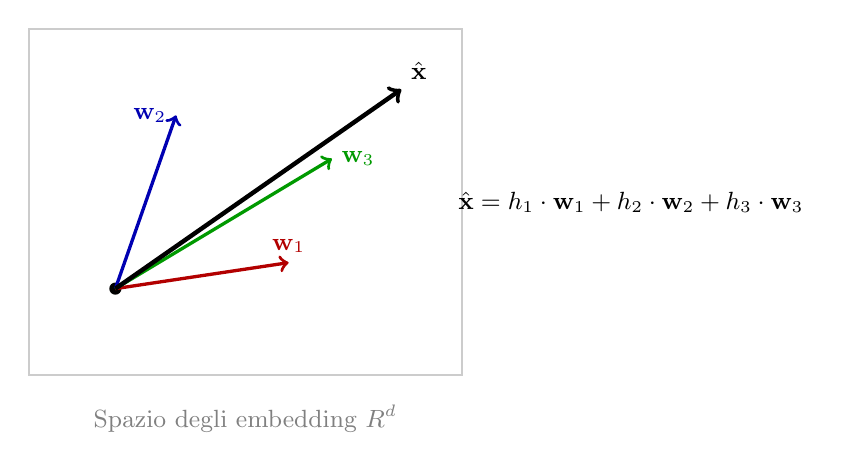
\begin{tikzpicture}[scale=1.1]
        % Spazio embedding
        \draw[thick, gray!40] (-0.5,-0.5) -- (4.5,-0.5) -- (4.5,3.5) -- (-0.5,3.5) -- cycle;
        \node[font=\small, gray] at (2, -1.0) {Spazio degli embedding $\mathbb{R}^d$};
        
        % Origine
        \fill[black] (0.5, 0.5) circle (2pt);
        
        % Vettori w_i (colonne del decoder)
        \draw[->, very thick, red!70!black] (0.5, 0.5) -- (2.5, 0.8);
        \node[above, font=\small, red!70!black] at (2.5, 0.8) {$\mathbf{w}_1$};
        
        \draw[->, very thick, blue!70!black] (0.5, 0.5) -- (1.2, 2.5);
        \node[left, font=\small, blue!70!black] at (1.2, 2.5) {$\mathbf{w}_2$};
        
        \draw[->, very thick, green!60!black] (0.5, 0.5) -- (3.0, 2.0);
        \node[right, font=\small, green!60!black] at (3.0, 2.0) {$\mathbf{w}_3$};
        
        % Vettore ricostruito (combinazione)
        \draw[->, ultra thick, black] (0.5, 0.5) -- (3.8, 2.8);
        \node[above right, font=\small\bfseries] at (3.8, 2.8) {$\hat{\mathbf{x}}$};
        
        % Equazione
        \node[font=\small, align=left] at (6.5, 1.5) {
            $\hat{\mathbf{x}} = h_1 \cdot \mathbf{w}_1 + h_2 \cdot \mathbf{w}_2 + h_3 \cdot \mathbf{w}_3$
        };
        
    \end{tikzpicture}
    \caption{La ricostruzione come combinazione lineare. Ogni colonna $\mathbf{w}_i$ della matrice del decoder rappresenta una direzione nello spazio degli embedding. La ricostruzione $\hat{\mathbf{x}}$ è la somma dei vettori $\mathbf{w}_i$ pesati dalle rispettive attivazioni $h_i$. La linearità garantisce che ogni feature contribuisca in modo indipendente e trasparente.}
    \label{fig:decoder_linear_combination}
\end{figure}

La linearità ha anche un'altra conseguenza importante: ogni colonna $\mathbf{w}_i$ può essere studiata in isolamento. Possiamo chiederci: ``quale direzione nello spazio degli embedding rappresenta la feature $i$?'' e rispondere ispezionando direttamente $\mathbf{w}_i$. Possiamo calcolare la similarità tra due feature confrontando $\mathbf{w}_i$ e $\mathbf{w}_j$. Possiamo persino intervenire sulla rappresentazione, aumentando o diminuendo un'attivazione $h_i$ per ``aggiungere'' o ``rimuovere'' una feature dalla ricostruzione. Nulla di tutto questo sarebbe possibile con un decoder non lineare.

\subsubsection{Feature come direzioni nello spazio degli embedding}
\label{subsubsec:features_as_directions}
Abbiamo stabilito che le colonne $\mathbf{w}_i$ della matrice del decoder rappresentano le feature apprese dal modello. Ma cosa significa, concretamente, che una feature è una ``direzione nello spazio degli embedding''?
Consideriamo lo spazio $\mathbb{R}^d$ in cui vivono gli embedding—ad esempio, lo spazio a 768 dimensioni di BERT. Ogni punto di questo spazio corrisponde a un possibile embedding, cioè alla rappresentazione di un testo. Punti vicini rappresentano testi semanticamente simili; punti lontani rappresentano testi dissimili. In questo spazio, una direzione non è semplicemente un punto, ma un \textit{asse lungo cui spostarsi}.
Ogni colonna $\mathbf{w}_i \in \mathbb{R}^d$ definisce una di queste direzioni. Muoversi lungo $\mathbf{w}_i$, partendo da un embedding $\mathbf{x}$, significa aggiungere o intensificare un certo aspetto semantico. Se $\mathbf{w}_{42}$ rappresenta il concetto di ``febbre'', allora:
\begin{equation}
    \mathbf{x}' = \mathbf{x} + \alpha \cdot \mathbf{w}_{42}
\end{equation}
produce un embedding $\mathbf{x}'$ in cui il concetto di febbre è più presente rispetto a $\mathbf{x}$. Il parametro $\alpha > 0$ controlla l'intensità di questa aggiunta. Questa è esattamente l'operazione che il decoder compie implicitamente: ricostruisce l'embedding sommando le direzioni delle feature attive, ciascuna pesata dalla propria attivazione.
Durante l'addestramento, le colonne di $W_d$ vengono tipicamente normalizzate a norma unitaria:
\begin{equation}
    \|\mathbf{w}_i\| = 1 \quad \forall i \in \{1, \dots, n\}
\end{equation}
Questa normalizzazione ha due scopi. Il primo è separare il ruolo della direzione da quello dell'intensità: $\mathbf{w}_i$ specifica \textit{quale} concetto, mentre $h_i$ specifica \textit{quanto} di quel concetto è presente. Senza normalizzazione, la stessa informazione potrebbe essere codificata sia nella norma di $\mathbf{w}_i$ che nel valore di $h_i$, creando ambiguità. Il secondo scopo è stabilizzare l'addestramento, evitando che alcune colonne crescano arbitrariamente a scapito di altre.

\begin{figure}[htbp]
    \centering
    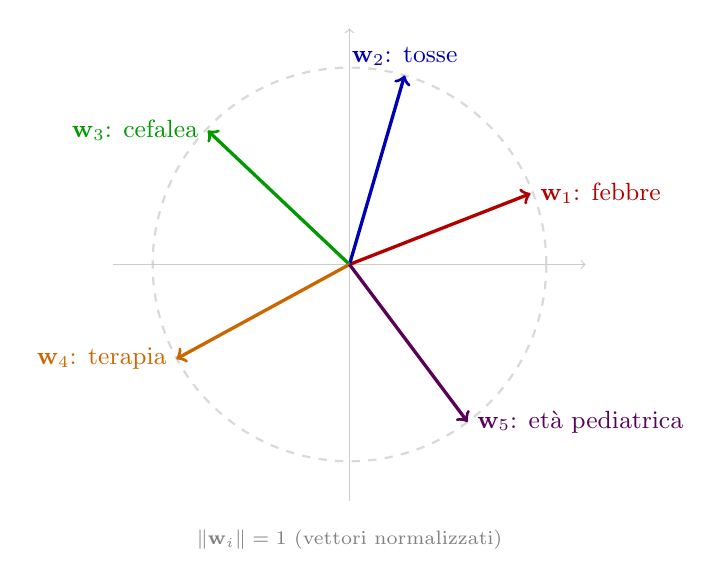
\begin{tikzpicture}[scale=1.0]
        % Cerchio unitario (per suggerire normalizzazione)
        \draw[thick, gray!30, dashed] (0,0) circle (2.5cm);
        
        % Assi di riferimento (grigi, sottili)
        \draw[gray!40, ->] (-3, 0) -- (3, 0);
        \draw[gray!40, ->] (0, -3) -- (0, 3);
        
        % Feature directions (normalizzate, sulla circonferenza)
        \draw[->, very thick, red!70!black] (0,0) -- (2.3, 0.9);
        \node[right, font=\small, red!70!black] at (2.3, 0.9) {$\mathbf{w}_1$: febbre};
        
        \draw[->, very thick, blue!70!black] (0,0) -- (0.7, 2.4);
        \node[above, font=\small, blue!70!black] at (0.7, 2.4) {$\mathbf{w}_2$: tosse};
        
        \draw[->, very thick, green!60!black] (0,0) -- (-1.8, 1.7);
        \node[left, font=\small, green!60!black] at (-1.8, 1.7) {$\mathbf{w}_3$: cefalea};
        
        \draw[->, very thick, orange!80!black] (0,0) -- (-2.2, -1.2);
        \node[left, font=\small, orange!80!black] at (-2.2, -1.2) {$\mathbf{w}_4$: terapia};
        
        \draw[->, very thick, violet!70!black] (0,0) -- (1.5, -2.0);
        \node[right, font=\small, violet!70!black] at (1.5, -2.0) {$\mathbf{w}_5$: età pediatrica};
        
        % Nota sulla normalizzazione
        \node[font=\scriptsize, gray] at (0, -3.5) {$\|\mathbf{w}_i\| = 1$ (vettori normalizzati)};
        
    \end{tikzpicture}
    \caption{Feature come direzioni normalizzate nello spazio degli embedding. Ogni colonna $\mathbf{w}_i$ del decoder definisce una direzione unitaria associata a un concetto semantico. Le direzioni non sono ortogonali: feature semanticamente correlate (come febbre e tosse) possono puntare in direzioni simili.}
    \label{fig:features_as_directions}
\end{figure}

È importante osservare che le direzioni $\mathbf{w}_i$ non sono, in generale, ortogonali tra loro. Questo potrebbe sembrare un fallimento: nel Capitolo~\ref{sec:04_disentangling_dense_embeddings_with_sparse_autoencoders} abbiamo presentato l'ortogonalità come condizione ideale per il disentanglement. Ma l'ortogonalità perfetta è impossibile quando il numero di feature $n$ supera la dimensionalità dello spazio $d$: in $\mathbb{R}^d$ possono esistere al massimo $d$ vettori mutuamente ortogonali. Con $n = 3072$ feature e $d = 768$ dimensioni, la non-ortogonalità è una necessità matematica.
Ciò che lo Sparse Autoencoder garantisce non è l'ortogonalità delle direzioni, ma la loro \textit{esplicitezza}. A differenza della superposition originaria—dove le direzioni erano sconosciute e mescolate—qui ogni $\mathbf{w}_i$ è un vettore ispezionabile, memorizzato come colonna della matrice $W_d$. Possiamo misurare il prodotto scalare $\mathbf{w}_i^T \mathbf{w}_j$ per quantificare la sovrapposizione tra due feature. Possiamo visualizzare le direzioni, confrontarle, raggrupparle. L'interferenza geometrica non è eliminata, ma è resa trasparente.
Questa trasparenza apre la strada all'interpretazione. Se $\mathbf{w}_i$ è una direzione nello spazio degli embedding, possiamo chiederci: quali testi producono embedding allineati con questa direzione? Ovvero: per quali input l'attivazione $h_i$ è elevata? La risposta a questa domanda—trovare i testi che ``accendono'' una feature—è il primo passo per assegnare un significato semantico alle direzioni apprese. Vedremo nella Sezione~\ref{subsec:interpretability} come questo processo possa essere automatizzato utilizzando un modello linguistico come interprete.
\begin{notebox}
\textbf{Riepilogo: l'architettura dello Sparse Autoencoder}\\
Lo Sparse Autoencoder trasforma un embedding denso $\mathbf{x} \in \mathbb{R}^d$ in una rappresentazione sparsa $\mathbf{h} \in \mathbb{R}^n$ con $n > d$:
\begin{itemize}
    \item L'\textbf{encoder} (non lineare) rileva quali feature sono presenti, producendo attivazioni $h_i \geq 0$
    \item Lo \textbf{spazio latente} è overcomplete: abbastanza dimensioni per rappresentare molte feature
    \item Il \textbf{decoder} (lineare) ricostruisce l'input come $\hat{\mathbf{x}} = \sum_i h_i \mathbf{w}_i + \mathbf{b}_d$
    \item Le \textbf{colonne} $\mathbf{w}_i$ di $W_d$ sono le direzioni delle feature, ispezionabili e interpretabili
\end{itemize}
La linearità del decoder è la chiave: garantisce che ogni feature contribuisca in modo indipendente e trasparente alla ricostruzione.
\end{notebox}

\subsection{Funzione di perdita e addestramento}
\label{subsec:loss_function}

L'architettura dello Sparse Autoencoder—encoder non lineare, spazio overcomplete, decoder lineare—definisce la struttura del modello. Ma è la funzione di perdita a determinare \textit{cosa} il modello apprende. In questa sezione esaminiamo i tre componenti della loss function e il loro ruolo nel produrre rappresentazioni sparse e interpretabili.

\subsubsection{La funzione di perdita complessiva}
\label{subsubsec:loss_overview}

L'obiettivo dell'addestramento è duplice: il modello deve ricostruire fedelmente gli embedding originali, ma deve farlo utilizzando rappresentazioni sparse. Questi due obiettivi sono potenzialmente in conflitto—una ricostruzione perfetta potrebbe richiedere molte feature attive simultaneamente—e la funzione di perdita deve bilanciarli.

Seguendo O'Neill et al.~\parencite{oneill2024disentangling}, la loss complessiva combina tre termini:
\begin{equation}
    \mathcal{L} = \mathcal{L}_{\text{rec}} + \lambda \mathcal{L}_{\text{sparse}}(\mathbf{h}) + \alpha \mathcal{L}_{\text{aux}}(\mathbf{x}, \hat{\mathbf{x}})
    \label{eq:total_loss}
\end{equation}
dove $\lambda > 0$ e $\alpha > 0$ sono iperparametri che controllano il peso relativo di ciascun termine.

Il primo termine è la \textbf{perdita di ricostruzione}, che misura quanto bene il decoder riesce a ricostruire l'input originale:
\begin{equation}
    \mathcal{L}_{\text{rec}} = \frac{1}{d} \|\mathbf{x} - \hat{\mathbf{x}}\|_2^2
    \label{eq:reconstruction_loss}
\end{equation}
Si tratta del Mean Squared Error (MSE) tra l'embedding originale $\mathbf{x}$ e la sua ricostruzione $\hat{\mathbf{x}}$, normalizzato per la dimensionalità $d$. Minimizzare questo termine spinge il modello a preservare l'informazione contenuta nell'embedding: una ricostruzione fedele implica che le feature estratte catturano gli aspetti rilevanti dell'input.

Il secondo termine è il \textbf{vincolo di sparsità}, che penalizza le rappresentazioni con troppe attivazioni non nulle:
\begin{equation}
    \mathcal{L}_{\text{sparse}}(\mathbf{h})
\end{equation}
La forma esatta di questo termine può variare; nella prossima sezione vedremo l'approccio Top-K adottato da O'Neill et al., che differisce dalla classica regolarizzazione $L_1$.
Il terzo termine è la \textbf{perdita ausiliaria}, introdotta per risolvere un problema pratico dell'addestramento—il fenomeno dei \textit{dead latents}:
\begin{equation}
    \mathcal{L}_{\text{aux}}(\mathbf{x}, \hat{\mathbf{x}})
\end{equation}
Dedicheremo la Sezione~\ref{subsubsec:auxiliary_loss} a questo componente. Il bilanciamento tra questi termini è cruciale. Se $\lambda$ è troppo basso, il modello potrebbe attivare molte feature per ogni input, perdendo il vantaggio della sparsità. Se $\lambda$ è troppo alto, il modello potrebbe sacrificare la qualità della ricostruzione pur di mantenere poche attivazioni. O'Neill et al. osservano che, con l'approccio Top-K, il coefficiente $\lambda$ diventa meno critico perché la sparsità è imposta come vincolo rigido piuttosto che come penalità morbida. Il coefficiente $\alpha$ della perdita ausiliaria è tipicamente fissato a $1/32$, un valore che bilancia l'effetto di recupero dei dead latents senza interferire eccessivamente con l'obiettivo principale.
\subsubsection{Il vincolo di sparsità Top-K}
\label{subsubsec:topk_sparsity}

L'approccio tradizionale per indurre sparsità in un autoencoder è la regolarizzazione $L_1$: aggiungere alla loss un termine proporzionale alla somma delle attivazioni:
\begin{equation}
    \mathcal{L}_{\text{sparse}}^{L_1}(\mathbf{h}) = \sum_{i=1}^{n} |h_i|
\end{equation}
Questo termine penalizza le attivazioni non nulle, spingendo il modello a utilizzare poche feature. Tuttavia, la regolarizzazione $L_1$ presenta un problema noto come \textit{shrinkage}: per ridurre la penalità, il modello tende a sottostimare sistematicamente le attivazioni, producendo valori $h_i$ più bassi di quelli che sarebbero ottimali per la ricostruzione~\parencite{oneill2024disentangling}. Il risultato è una rappresentazione sì sparsa, ma anche meno fedele.
O'Neill et al. adottano un approccio diverso: il vincolo \textbf{Top-K} (o \textit{k-sparse})~\parencite{makhzani2013ksparse}. Invece di penalizzare le attivazioni con un termine morbido, si impone un vincolo rigido: per ogni input, solo le $k$ attivazioni più grandi vengono mantenute, mentre tutte le altre sono forzate a zero.
Formalmente, sia $\mathbf{z} = W_e \mathbf{x} + \mathbf{b}_e$ il vettore delle pre-attivazioni. Il vincolo Top-K opera in due passi:
\begin{enumerate}
    \item Si identificano gli indici delle $k$ componenti di $\mathbf{z}$ con valore più alto
    \item Si pongono a zero tutte le altre componenti
\end{enumerate}
L'attivazione finale è quindi:
\begin{equation}
    h_i = \begin{cases}
        \sigma(z_i) & \text{se } z_i \text{ è tra i } k \text{ valori più alti} \\
        0 & \text{altrimenti}
    \end{cases}
    \label{eq:topk_activation}
\end{equation}
dove $\sigma(\cdot)$ è la ReLU.

\begin{figure}[htbp]
    \centering
    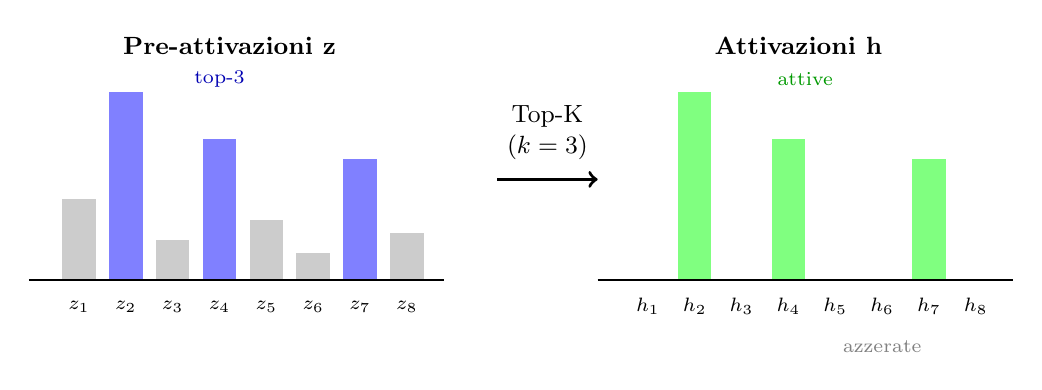
\begin{tikzpicture}[scale=0.85]
        
        % === Pre-attivazioni z ===
        \node[font=\small\bfseries] at (0, 3.5) {Pre-attivazioni $\mathbf{z}$};
        
        % Barre delle pre-attivazioni
        \fill[gray!40] (-2.5, 0) rectangle (-2.0, 1.2);
        \fill[blue!50] (-1.8, 0) rectangle (-1.3, 2.8);
        \fill[gray!40] (-1.1, 0) rectangle (-0.6, 0.6);
        \fill[blue!50] (-0.4, 0) rectangle (0.1, 2.1);
        \fill[gray!40] (0.3, 0) rectangle (0.8, 0.9);
        \fill[gray!40] (1.0, 0) rectangle (1.5, 0.4);
        \fill[blue!50] (1.7, 0) rectangle (2.2, 1.8);
        \fill[gray!40] (2.4, 0) rectangle (2.9, 0.7);
        
        % Asse
        \draw[thick] (-3, 0) -- (3.2, 0);
        
        % Labels
        \node[font=\scriptsize] at (-2.25, -0.4) {$z_1$};
        \node[font=\scriptsize] at (-1.55, -0.4) {$z_2$};
        \node[font=\scriptsize] at (-0.85, -0.4) {$z_3$};
        \node[font=\scriptsize] at (-0.15, -0.4) {$z_4$};
        \node[font=\scriptsize] at (0.55, -0.4) {$z_5$};
        \node[font=\scriptsize] at (1.25, -0.4) {$z_6$};
        \node[font=\scriptsize] at (1.95, -0.4) {$z_7$};
        \node[font=\scriptsize] at (2.65, -0.4) {$z_8$};
        
        % Freccia Top-K
        \draw[->, very thick] (4, 1.5) -- (5.5, 1.5);
        \node[font=\small, align=center] at (4.75, 2.2) {Top-K\\($k=3$)};
        
        % === Attivazioni h ===
        \node[font=\small\bfseries] at (8.5, 3.5) {Attivazioni $\mathbf{h}$};
        
        % Barre delle attivazioni (solo top-k)
        \fill[gray!20] (6.0, 0) rectangle (6.5, 0);
        \fill[green!50] (6.7, 0) rectangle (7.2, 2.8);
        \fill[gray!20] (7.4, 0) rectangle (7.9, 0);
        \fill[green!50] (8.1, 0) rectangle (8.6, 2.1);
        \fill[gray!20] (8.8, 0) rectangle (9.3, 0);
        \fill[gray!20] (9.5, 0) rectangle (10.0, 0);
        \fill[green!50] (10.2, 0) rectangle (10.7, 1.8);
        \fill[gray!20] (10.9, 0) rectangle (11.4, 0);
        
        % Asse
        \draw[thick] (5.5, 0) -- (11.7, 0);
        
        % Labels
        \node[font=\scriptsize] at (6.25, -0.4) {$h_1$};
        \node[font=\scriptsize] at (6.95, -0.4) {$h_2$};
        \node[font=\scriptsize] at (7.65, -0.4) {$h_3$};
        \node[font=\scriptsize] at (8.35, -0.4) {$h_4$};
        \node[font=\scriptsize] at (9.05, -0.4) {$h_5$};
        \node[font=\scriptsize] at (9.75, -0.4) {$h_6$};
        \node[font=\scriptsize] at (10.45, -0.4) {$h_7$};
        \node[font=\scriptsize] at (11.15, -0.4) {$h_8$};
        
        % Annotazioni
        \node[font=\scriptsize, blue!70!black] at (-0.15, 3.0) {top-3};
        \node[font=\scriptsize, green!60!black] at (8.6, 3.0) {attive};
        \node[font=\scriptsize, gray] at (9.75, -1.0) {azzerate};
        
    \end{tikzpicture}
    \caption{Il vincolo Top-K. A sinistra: le pre-attivazioni $\mathbf{z}$ calcolate dall'encoder. Le tre componenti con valore più alto sono evidenziate in blu. A destra: le attivazioni finali $\mathbf{h}$ dopo l'applicazione del vincolo Top-K con $k=3$. Solo le componenti selezionate (in verde) mantengono il loro valore; tutte le altre sono forzate a zero.}
    \label{fig:topk_mechanism}
\end{figure}

Il vantaggio del Top-K rispetto alla regolarizzazione $L_1$ è duplice. 

Il primo vantaggio è l'assenza di shrinkage. Le $k$ attivazioni selezionate mantengono il loro valore originale $\sigma(z_i)$, senza alcuna penalizzazione. Il modello può quindi apprendere attivazioni di intensità appropriata senza il compromesso imposto dalla regolarizzazione.

Il secondo vantaggio è il controllo diretto sulla sparsità. Con $L_1$, il livello di sparsità dipende dal coefficiente $\lambda$ e deve essere calibrato empiricamente. Con Top-K, la sparsità è deterministica: esattamente $k$ feature attive per input, né più né meno. Questo rende il comportamento del modello più prevedibile e i risultati più riproducibili.

La scelta del valore di $k$ è un iperparametro cruciale. Valori tipici variano tra 16 e 128, a seconda della complessità del dominio e della granularità desiderata~\parencite{oneill2024disentangling}. Un $k$ più basso produce rappresentazioni più sparse ma potenzialmente meno accurate; un $k$ più alto permette ricostruzioni migliori ma con meno separazione tra le feature. O'Neill et al. esplorano tre configurazioni principali:
\begin{itemize}
    \item \textbf{SAE16}: $k = 16$ attivazioni, $n = 2d = 3072$ feature totali
    \item \textbf{SAE32}: $k = 32$ attivazioni, $n = 4d = 6144$ feature totali
    \item \textbf{SAE64}: $k = 64$ attivazioni, $n = 6d = 9216$ feature totali
\end{itemize}
All'aumentare di $k$ e $n$, le feature apprese tendono a diventare più granulari e specifiche—un fenomeno che esploreremo nella Sezione~\ref{subsec:feature_splitting}.


\subsubsection{Auxiliary loss e il problema dei dead latents}
\label{subsubsec:auxiliary_loss}

Durante l'addestramento di uno Sparse Autoencoder può emergere un problema insidioso: alcune feature smettono di attivarsi completamente. Il vincolo Top-K seleziona, per ogni input, solo le $k$ attivazioni più alte; se una feature produce sistematicamente valori bassi, non verrà mai selezionata e i suoi parametri smetteranno di ricevere gradienti. Senza gradienti, la feature non può migliorare; senza miglioramento, continuerà a produrre valori bassi. Si innesca un circolo vizioso che porta la feature a ``morire''.

Queste feature inutilizzate sono chiamate \textbf{dead latents}. O'Neill et al.~\parencite{oneill2024disentangling} definiscono operativamente un latent come ``morto'' se non si è attivato per un'intera epoca di addestramento. Il problema non è solo teorico: nei primi esperimenti con SAE a $k=16$, gli autori osservano che una frazione significativa delle feature può diventare inattiva durante il training (Figura~\ref{fig:dead_latents}).

\begin{figure}[htbp]
    \centering
    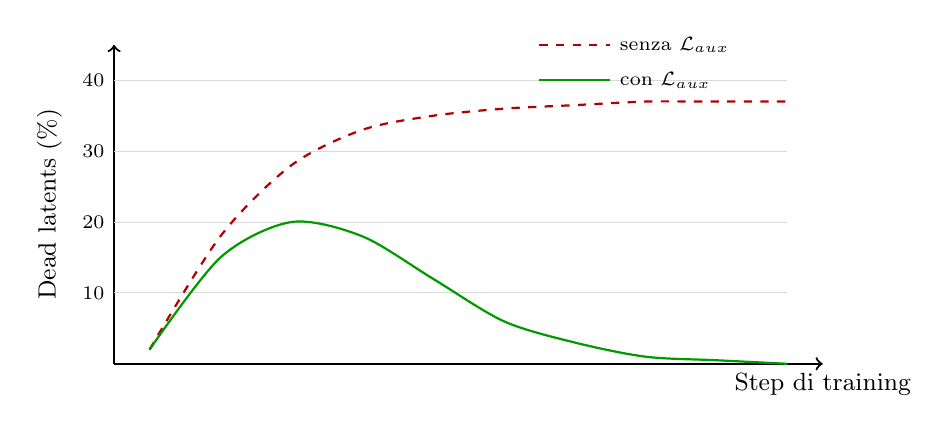
\begin{tikzpicture}[scale=0.9]
        % Asse x
        \draw[->, thick] (0, 0) -- (10, 0);
        \node[below, font=\small] at (10, 0) {Step di training};
        
        % Asse y
        \draw[->, thick] (0, 0) -- (0, 4.5);
        \node[above, rotate=90, font=\small] at (-0.6, 2.25) {Dead latents (\%)};
        
        % Griglia
        \draw[gray!30, thin] (0, 1) -- (9.5, 1);
        \draw[gray!30, thin] (0, 2) -- (9.5, 2);
        \draw[gray!30, thin] (0, 3) -- (9.5, 3);
        \draw[gray!30, thin] (0, 4) -- (9.5, 4);
        
        % Labels asse y
        \node[left, font=\scriptsize] at (0, 1) {10};
        \node[left, font=\scriptsize] at (0, 2) {20};
        \node[left, font=\scriptsize] at (0, 3) {30};
        \node[left, font=\scriptsize] at (0, 4) {40};
        
        % Curva (senza auxiliary loss)
        \draw[thick, red!70!black, dashed] plot[smooth] coordinates {
            (0.5, 0.2) (1.5, 1.8) (2.5, 2.8) (3.5, 3.3) (4.5, 3.5) (5.5, 3.6) (6.5, 3.65) (7.5, 3.7) (8.5, 3.7) (9.5, 3.7)
        };
        
        % Curva (con auxiliary loss)
        \draw[thick, green!60!black] plot[smooth] coordinates {
            (0.5, 0.2) (1.5, 1.5) (2.5, 2.0) (3.5, 1.8) (4.5, 1.2) (5.5, 0.6) (6.5, 0.3) (7.5, 0.1) (8.5, 0.05) (9.5, 0)
        };
        
        % Legenda
        \draw[thick, red!70!black, dashed] (6, 4.5) -- (7, 4.5);
        \node[right, font=\scriptsize] at (7, 4.5) {senza $\mathcal{L}_{\text{aux}}$};
        
        \draw[thick, green!60!black] (6, 4) -- (7, 4);
        \node[right, font=\scriptsize] at (7, 4) {con $\mathcal{L}_{\text{aux}}$};
        
    \end{tikzpicture}
    \caption{Evoluzione dei dead latents durante il training (illustrazione qualitativa basata sui risultati di O'Neill et al.). Senza la perdita ausiliaria, una frazione significativa di feature diventa permanentemente inattiva. Con la perdita ausiliaria, i dead latents vengono progressivamente ``rianimati'' fino a scomparire.}
    \label{fig:dead_latents}
\end{figure}
I dead latents rappresentano uno spreco di capacità. Se il modello ha $n = 3072$ feature ma 500 sono morte, la capacità effettiva si riduce a 2572 feature—vanificando parte del vantaggio dell'overcompletezza. Peggio ancora, le feature che sopravvivono potrebbero essere costrette a rappresentare più concetti di quanti ne potrebbero gestire, reintroducendo una forma di polisemantictà.
Per contrastare questo fenomeno, O'Neill et al. introducono una \textbf{perdita ausiliaria} ispirata alla tecnica dei ``ghost grads''~\parencite{jermyn2023ghostgrads}. L'idea è semplice: se una feature è morta, non riceve gradienti dalla loss principale perché non contribuisce alla ricostruzione. Ma possiamo \textit{forzarla} a contribuire chiedendole di ricostruire l'\textit{errore} del modello.
Formalmente, sia $\mathbf{e} = \mathbf{x} - \hat{\mathbf{x}}$ l'errore di ricostruzione del modello principale. La perdita ausiliaria chiede ai dead latents di modellare questo errore:
\begin{equation}
    \mathcal{L}_{\text{aux}}(\mathbf{x}, \hat{\mathbf{x}}) = \|\mathbf{e} - \hat{\mathbf{e}}\|_2^2
    \label{eq:auxiliary_loss}
\end{equation}
dove $\hat{\mathbf{e}} = W_d \mathbf{z}$ è la ricostruzione dell'errore ottenuta usando solo i dead latents. Il vettore $\mathbf{z}$ è una rappresentazione sparsa che utilizza esclusivamente le $k_{\text{aux}}$ feature attualmente inattive con le pre-attivazioni più alte.
Il meccanismo funziona così: le feature ``vive'' ricostruiscono $\mathbf{x}$ producendo $\hat{\mathbf{x}}$; le feature ``morte'' cercano di ricostruire l'errore residuo $\mathbf{e}$. Se un dead latent riesce a catturare parte dell'errore, la sua direzione $\mathbf{w}_i$ sta evidentemente codificando informazione utile che le feature attive non stanno rappresentando. Il gradiente della perdita ausiliaria ``risveglia'' questo latent, dandogli la possibilità di competere nuovamente per essere selezionato dal Top-K.
\begin{notebox}
\textbf{Il meccanismo della perdita ausiliaria}\\
\begin{enumerate}
    \item Le feature attive ricostruiscono l'input: $\hat{\mathbf{x}} = \sum_{i \in \text{attive}} h_i \mathbf{w}_i + \mathbf{b}_d$
    \item Si calcola l'errore residuo: $\mathbf{e} = \mathbf{x} - \hat{\mathbf{x}}$
    \item I dead latents cercano di ricostruire l'errore: $\hat{\mathbf{e}} = \sum_{j \in \text{morti}} z_j \mathbf{w}_j$
    \item Se ci riescono, ricevono gradienti e possono ``tornare in vita''
\end{enumerate}
\end{notebox}
Il parametro $k_{\text{aux}}$ controlla quanti dead latents vengono coinvolti in ogni step. O'Neill et al. utilizzano tipicamente $k_{\text{aux}} = 2k$: il doppio dei latenti attivi nel modello principale. Il coefficiente $\alpha$ nella loss complessiva (Equazione~\ref{eq:total_loss}) è fissato a $1/32$, un valore sufficientemente basso da non interferire con l'obiettivo principale di ricostruzione, ma abbastanza alto da garantire il recupero dei dead latents nel corso dell'addestramento.
L'efficacia di questa tecnica è notevole. O'Neill et al. riportano che, alla fine del training, tutti i modelli presentano zero dead latents—tutte le $n$ feature hanno imparato a contribuire alla rappresentazione. Questo risultato è particolarmente importante per l'interpretabilità: significa che l'intera capacità del modello è effettivamente utilizzata, e ogni direzione $\mathbf{w}_i$ nel decoder rappresenta potenzialmente un concetto distinto.
\subsection{Interpretabilità automatica delle feature}
\label{subsec:interpretability}
Lo Sparse Autoencoder produce una rappresentazione in cui ogni feature corrisponde a una direzione $\mathbf{w}_i$ nello spazio degli embedding e a un'attivazione $h_i$ che ne indica l'intensità. Ma una direzione geometrica, di per sé, non è interpretabile: per rendere le feature comprensibili agli esseri umani, dobbiamo associare a ciascuna un'etichetta semantica—un nome che descriva il concetto che quella feature cattura.
Un approccio manuale sarebbe impraticabile. Con migliaia di feature ($n = 3072$ o più), ispezionare una per una i testi che le attivano richiederebbe settimane di lavoro. O'Neill et al.~\parencite{oneill2024disentangling} propongono invece un approccio automatizzato: utilizzare un Large Language Model come \textbf{interprete} delle feature.
\subsubsection{L'Interpreter LLM}
\label{subsubsec:interpreter}
L'intuizione è semplice. Se una feature cattura un concetto semantico coerente, i testi che la attivano fortemente dovrebbero condividere qualcosa—un tema, un argomento, una proprietà stilistica. Un modello linguistico, esaminando questi testi, dovrebbe essere in grado di identificare il denominatore comune.
Il processo di interpretazione si articola in tre passi:
\textbf{Passo 1: Identificare i testi attivanti.} Per ogni feature $i$, si scorre l'intero corpus di documenti e si calcolano le attivazioni $h_i$ prodotte dall'encoder. Si selezionano i $k$ documenti con le attivazioni più alte—i testi che ``accendono'' maggiormente quella feature. Tipicamente $k = 5$.
\textbf{Passo 2: Identificare i contro-esempi.} Si selezionano anche alcuni documenti che \textit{non} attivano la feature ($h_i = 0$). Questi contro-esempi aiutano l'interprete a discriminare: il concetto cercato deve essere presente nei testi attivanti e assente nei contro-esempi.
\textbf{Passo 3: Interrogare l'LLM.} I testi attivanti e i contro-esempi vengono forniti a un modello linguistico insieme a un prompt che chiede di identificare il tema comune. L'LLM restituisce un'etichetta breve (1-8 parole) che descrive la feature.

\begin{figure}[htbp]
    \centering
    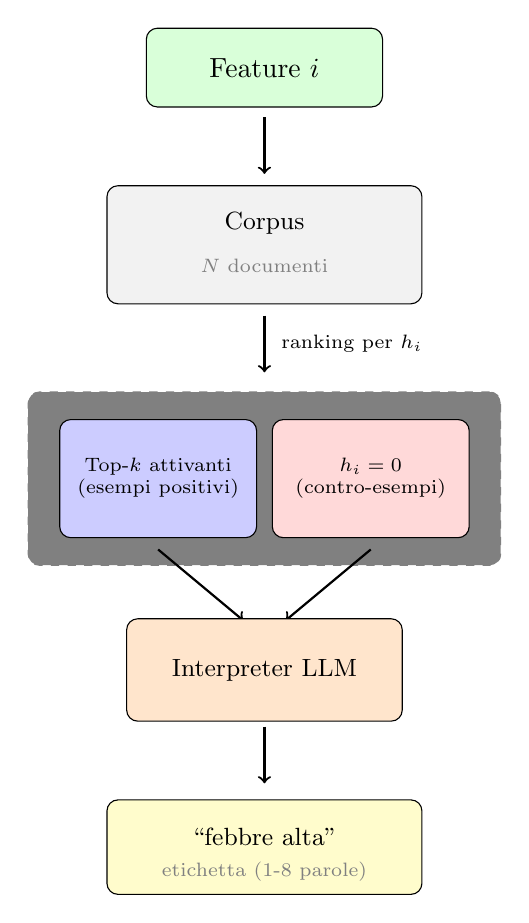
\begin{tikzpicture}[scale=0.9]
        
        % Feature box (top)
        \node[draw, rectangle, minimum width=3cm, minimum height=1cm, fill=green!15, rounded corners] (feature) at (0, 0) {Feature $i$};
        
        % Freccia verso corpus
        \draw[->, thick] (0, -0.7) -- (0, -1.5);
        
        % Corpus
        \node[draw, rectangle, minimum width=4cm, minimum height=1.5cm, fill=gray!10, rounded corners] (corpus) at (0, -2.5) {};
        \node[font=\small] at (0, -2.2) {Corpus};
        \node[font=\scriptsize, gray] at (0, -2.8) {$N$ documenti};
        
        % Freccia verso selezione
        \draw[->, thick] (0, -3.5) -- (0, -4.3);
        \node[right, font=\scriptsize] at (0.1, -3.9) {ranking per $h_i$};
        
        % Box contenitore per esempi
        \node[draw, rectangle, minimum width=6cm, minimum height=2.2cm, fill=white, rounded corners, dashed, gray] at (0, -5.8) {};
        
        % Testi attivanti (sinistra)
        \node[draw, rectangle, minimum width=2.5cm, minimum height=1.5cm, fill=blue!20, rounded corners] (pos) at (-1.5, -5.8) {};
        \node[font=\scriptsize, align=center] at (-1.5, -5.8) {Top-$k$ attivanti\\(esempi positivi)};
        
        % Testi non attivanti (destra)
        \node[draw, rectangle, minimum width=2.5cm, minimum height=1.5cm, fill=red!15, rounded corners] (neg) at (1.5, -5.8) {};
        \node[font=\scriptsize, align=center] at (1.5, -5.8) {$h_i = 0$\\(contro-esempi)};
        
        % Frecce verso LLM
        \draw[->, thick] (-1.5, -6.8) -- (-0.3, -7.8);
        \draw[->, thick] (1.5, -6.8) -- (0.3, -7.8);
        
        % LLM
        \node[draw, rectangle, minimum width=3.5cm, minimum height=1.3cm, fill=orange!20, rounded corners] (llm) at (0, -8.5) {};
        \node[font=\small, align=center] at (0, -8.5) {Interpreter LLM};
        
        % Freccia verso output
        \draw[->, thick] (0, -9.3) -- (0, -10.1);
        
        % Output
        \node[draw, rectangle, minimum width=4cm, minimum height=1.2cm, fill=yellow!20, rounded corners] (label) at (0, -11) {};
        \node[font=\small, align=center] at (0, -10.85) {``febbre alta''};
        \node[font=\scriptsize, gray] at (0, -11.35) {etichetta (1-8 parole)};
        
    \end{tikzpicture}
    \caption{Il processo di interpretazione automatica. Per ogni feature, si identificano i testi che la attivano maggiormente e quelli che non la attivano affatto. Un LLM esamina entrambi gli insiemi e produce un'etichetta che descrive il concetto catturato dalla feature.}
    \label{fig:interpreter_process}
\end{figure}

Il prompt fornito all'interprete è progettato con cura. O'Neill et al. istruiscono il modello a comportarsi come un ``meticoloso ricercatore'' che deve scoprire quale comportamento attiva un certo neurone. Il prompt richiede di:
\begin{enumerate}
    \item Elencare i potenziali temi comuni tra i testi attivanti, a diversi livelli di granularità
    \item Escludere i temi presenti anche nei contro-esempi
    \item Applicare il rasoio di Occam: scegliere la spiegazione più semplice compatibile con i dati
    \item Formulare l'etichetta finale in 1-8 parole
\end{enumerate}
Il riferimento al rasoio di Occam è particolarmente importante. Senza questa indicazione, l'interprete potrebbe produrre etichette troppo specifiche (che catturano solo un sottoinsieme dei testi attivanti) o troppo generiche (che non discriminano dai contro-esempi). La richiesta di semplicità guida verso etichette al giusto livello di astrazione.
\subsubsection{Implementazione in PRISMA}
\label{subsubsec:prisma_interpreter}
In PRISMA, l'interpretazione delle feature è implementata attraverso l'integrazione con Ollama, un framework per l'esecuzione locale di modelli linguistici. Questa scelta presenta vantaggi significativi: non richiede connessione a servizi cloud, garantisce la privacy dei dati (particolarmente importante nel contesto medico), e permette di processare grandi volumi di feature senza costi di API.
Il processo segue fedelmente lo schema descritto sopra. Per ogni feature del SAE addestrato:
\begin{enumerate}
    \item Il modulo \texttt{explorer} scansiona tutti i documenti del corpus
    \item Identifica i documenti con le attivazioni più alte per quella feature
    \item Seleziona documenti con attivazione nulla come contro-esempi
    \item Costruisce il prompt con esempi positivi e negativi
    \item Invia la richiesta al modello locale via Ollama
    \item Memorizza l'etichetta risultante nel database
\end{enumerate}

Il prompt utilizzato in PRISMA è adattato al dominio medico-pediatrico. L'LLM viene istruito a cercare concetti clinici specifici—sintomi, diagnosi, trattamenti, fasce d'età—piuttosto che temi generici. Questa specializzazione migliora la qualità delle etichette nel dominio di applicazione.

\begin{notebox}
\textbf{Esempio di interpretazione}\\
Supponiamo che una feature si attivi fortemente sui seguenti testi:
\begin{itemize}
    \item ``Paziente presenta temperatura corporea 39.2°C''
    \item ``Febbre persistente da tre giorni, non responsiva a paracetamolo''
    \item ``Iperpiressia in paziente pediatrico di 4 anni''
\end{itemize}
E non si attivi su:
\begin{itemize}
    \item ``Esame obiettivo nella norma, paziente apiretico''
    \item ``Tosse secca senza rialzo termico''
\end{itemize}
L'interprete, confrontando i due insiemi, identificherebbe il tema comune e produrrebbe l'etichetta: ``febbre / iperpiressia''.
\end{notebox}
È importante sottolineare i limiti di questo approccio. L'interpretazione automatica è un'euristica, non una dimostrazione formale che la feature catturi esattamente il concetto indicato dall'etichetta. Alcune feature potrebbero essere polisemantiche (catturare più concetti correlati), altre potrebbero essere difficili da descrivere in poche parole. O'Neill et al. propongono un secondo passo—un \textit{Predictor} LLM che valida le etichette predicendo le attivazioni su testi unseen—ma questa validazione formale esula dagli scopi dell'implementazione attuale di PRISMA. Le etichette vanno quindi intese come ipotesi interpretative da verificare qualitativamente, non come verità assolute.
\subsection{Analisi della struttura delle feature}
\label{subsec:feature_analysis}
Le feature apprese da uno Sparse Autoencoder non sono entità isolate. L'analisi empirica rivela che si organizzano in strutture ricche: alcune feature tendono ad attivarsi insieme (\textit{feature families}), altre emergono come specializzazioni di feature più generali al crescere della capacità del modello (\textit{feature splitting}). Per studiare queste strutture in modo rigoroso, introduciamo un insieme di matrici che catturano diversi aspetti del comportamento delle feature.
\subsubsection{Notazione e matrici fondamentali}
\label{subsubsec:notation_matrices}
Sia $N$ il numero di documenti nel corpus e $n$ il numero di feature dello Sparse Autoencoder. Quando confrontiamo SAE di dimensioni diverse, indicheremo con $n_1$ e $n_2$ i rispettivi numeri di feature.
\paragraph{Matrice delle attivazioni.} La \textbf{matrice delle attivazioni} $H \in \mathbb{R}^{N \times n}$ raccoglie le attivazioni di tutte le feature su tutti i documenti:
\begin{equation}
    H_{ki} = h_{k,i} = \left[ f_\theta(\mathbf{x}_k) \right]_i
    \label{eq:activation_matrix}
\end{equation}
dove $h_{k,i}$ è l'attivazione della feature $i$ sul documento $k$, ottenuta passando l'embedding $\mathbf{x}_k$ attraverso l'encoder $f_\theta$. Ogni riga di $H$ è il vettore latente sparso di un documento; ogni colonna rappresenta il pattern di attivazione di una feature sull'intero corpus.
Grazie al vincolo Top-K, la matrice $H$ è intrinsecamente sparsa: per ogni riga, al massimo $k$ elementi sono non nulli. Seguendo O'Neill et al.~\parencite{oneill2024disentangling}, utilizziamo anche la notazione $B \equiv H$ quando vogliamo enfatizzare che stiamo considerando i \textit{valori} delle attivazioni (non solo la loro presenza).
\paragraph{Matrice delle attivazioni binaria.} La \textbf{matrice binaria} $A \in \{0,1\}^{N \times n}$ indica semplicemente se una feature è attiva o meno:
\begin{equation}
    A_{ki} = \chi_{H_{ki} > 0} = 
    \begin{cases}
        1 & \text{se la feature } i \text{ è attiva sul documento } k \\
        0 & \text{altrimenti}
    \end{cases}
    \label{eq:binary_activation}
\end{equation}
dove $\chi$ è la funzione caratteristica. Una feature è considerata ``attiva'' quando la sua attivazione è non nulla---ovvero quando è stata selezionata dal meccanismo Top-K.
\begin{figure}[htbp]
    \centering
    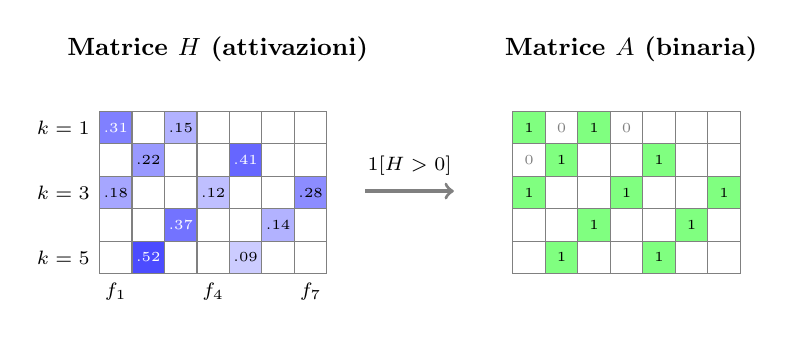
\begin{tikzpicture}[scale=0.75]
        
        % Matrice H
        \node[font=\small\bfseries] at (2, 3.8) {Matrice $H$ (attivazioni)};
        
        \def\rows{5}
        \def\cols{7}
        \def\cellsize{0.55}
        
        % Celle con valori
        % Doc 1
        \fill[blue!50] (0*\cellsize, 4*\cellsize) rectangle (1*\cellsize, 5*\cellsize);
        \node[font=\tiny, white] at (0.5*\cellsize, 4.5*\cellsize) {.31};
        \fill[blue!30] (2*\cellsize, 4*\cellsize) rectangle (3*\cellsize, 5*\cellsize);
        \node[font=\tiny] at (2.5*\cellsize, 4.5*\cellsize) {.15};
        
        % Doc 2
        \fill[blue!40] (1*\cellsize, 3*\cellsize) rectangle (2*\cellsize, 4*\cellsize);
        \node[font=\tiny] at (1.5*\cellsize, 3.5*\cellsize) {.22};
        \fill[blue!60] (4*\cellsize, 3*\cellsize) rectangle (5*\cellsize, 4*\cellsize);
        \node[font=\tiny, white] at (4.5*\cellsize, 3.5*\cellsize) {.41};
        
        % Doc 3
        \fill[blue!35] (0*\cellsize, 2*\cellsize) rectangle (1*\cellsize, 3*\cellsize);
        \node[font=\tiny] at (0.5*\cellsize, 2.5*\cellsize) {.18};
        \fill[blue!25] (3*\cellsize, 2*\cellsize) rectangle (4*\cellsize, 3*\cellsize);
        \node[font=\tiny] at (3.5*\cellsize, 2.5*\cellsize) {.12};
        \fill[blue!45] (6*\cellsize, 2*\cellsize) rectangle (7*\cellsize, 3*\cellsize);
        \node[font=\tiny] at (6.5*\cellsize, 2.5*\cellsize) {.28};
        
        % Doc 4
        \fill[blue!55] (2*\cellsize, 1*\cellsize) rectangle (3*\cellsize, 2*\cellsize);
        \node[font=\tiny, white] at (2.5*\cellsize, 1.5*\cellsize) {.37};
        \fill[blue!30] (5*\cellsize, 1*\cellsize) rectangle (6*\cellsize, 2*\cellsize);
        \node[font=\tiny] at (5.5*\cellsize, 1.5*\cellsize) {.14};
        
        % Doc 5
        \fill[blue!70] (1*\cellsize, 0*\cellsize) rectangle (2*\cellsize, 1*\cellsize);
        \node[font=\tiny, white] at (1.5*\cellsize, 0.5*\cellsize) {.52};
        \fill[blue!20] (4*\cellsize, 0*\cellsize) rectangle (5*\cellsize, 1*\cellsize);
        \node[font=\tiny] at (4.5*\cellsize, 0.5*\cellsize) {.09};
        
        % Griglia
        \draw[gray, thin] (0, 0) grid[step=\cellsize] (\cols*\cellsize, \rows*\cellsize);
        
        % Labels
        \node[left, font=\scriptsize] at (0, 4.5*\cellsize) {$k=1$};
        \node[left, font=\scriptsize] at (0, 2.5*\cellsize) {$k=3$};
        \node[left, font=\scriptsize] at (0, 0.5*\cellsize) {$k=5$};
        \node[below, font=\scriptsize] at (0.5*\cellsize, 0) {$f_1$};
        \node[below, font=\scriptsize] at (3.5*\cellsize, 0) {$f_4$};
        \node[below, font=\scriptsize] at (6.5*\cellsize, 0) {$f_7$};
        
        % Freccia
        \draw[->, very thick, gray] (4.5, 1.4) -- (6, 1.4);
        \node[above, font=\scriptsize] at (5.25, 1.5) {$\mathbb{1}[H > 0]$};
        
        % Matrice A
        \begin{scope}[shift={(7, 0)}]
            \node[font=\small\bfseries] at (2, 3.8) {Matrice $A$ (binaria)};
            
            % Doc 1
            \fill[green!50] (0*\cellsize, 4*\cellsize) rectangle (1*\cellsize, 5*\cellsize);
            \node[font=\tiny] at (0.5*\cellsize, 4.5*\cellsize) {1};
            \fill[green!50] (2*\cellsize, 4*\cellsize) rectangle (3*\cellsize, 5*\cellsize);
            \node[font=\tiny] at (2.5*\cellsize, 4.5*\cellsize) {1};
            
            % Doc 2
            \fill[green!50] (1*\cellsize, 3*\cellsize) rectangle (2*\cellsize, 4*\cellsize);
            \node[font=\tiny] at (1.5*\cellsize, 3.5*\cellsize) {1};
            \fill[green!50] (4*\cellsize, 3*\cellsize) rectangle (5*\cellsize, 4*\cellsize);
            \node[font=\tiny] at (4.5*\cellsize, 3.5*\cellsize) {1};
            
            % Doc 3
            \fill[green!50] (0*\cellsize, 2*\cellsize) rectangle (1*\cellsize, 3*\cellsize);
            \node[font=\tiny] at (0.5*\cellsize, 2.5*\cellsize) {1};
            \fill[green!50] (3*\cellsize, 2*\cellsize) rectangle (4*\cellsize, 3*\cellsize);
            \node[font=\tiny] at (3.5*\cellsize, 2.5*\cellsize) {1};
            \fill[green!50] (6*\cellsize, 2*\cellsize) rectangle (7*\cellsize, 3*\cellsize);
            \node[font=\tiny] at (6.5*\cellsize, 2.5*\cellsize) {1};
            
            % Doc 4
            \fill[green!50] (2*\cellsize, 1*\cellsize) rectangle (3*\cellsize, 2*\cellsize);
            \node[font=\tiny] at (2.5*\cellsize, 1.5*\cellsize) {1};
            \fill[green!50] (5*\cellsize, 1*\cellsize) rectangle (6*\cellsize, 2*\cellsize);
            \node[font=\tiny] at (5.5*\cellsize, 1.5*\cellsize) {1};
            
            % Doc 5
            \fill[green!50] (1*\cellsize, 0*\cellsize) rectangle (2*\cellsize, 1*\cellsize);
            \node[font=\tiny] at (1.5*\cellsize, 0.5*\cellsize) {1};
            \fill[green!50] (4*\cellsize, 0*\cellsize) rectangle (5*\cellsize, 1*\cellsize);
            \node[font=\tiny] at (4.5*\cellsize, 0.5*\cellsize) {1};
            
            % Zeri espliciti in alcune celle vuote
            \node[font=\tiny, gray] at (1.5*\cellsize, 4.5*\cellsize) {0};
            \node[font=\tiny, gray] at (3.5*\cellsize, 4.5*\cellsize) {0};
            \node[font=\tiny, gray] at (0.5*\cellsize, 3.5*\cellsize) {0};
            
            % Griglia
            \draw[gray, thin] (0, 0) grid[step=\cellsize] (\cols*\cellsize, \rows*\cellsize);
        \end{scope}
        
    \end{tikzpicture}
    \caption{Dalla matrice delle attivazioni $H$ alla matrice binaria $A$. A sinistra: $H$ contiene i valori continui delle attivazioni (le celle vuote sono zeri, dovuti al vincolo Top-K). A destra: $A$ indica solo se una feature è attiva (1) o meno (0). La sparsità è evidente: ogni riga ha al massimo $k$ elementi non nulli.}
    \label{fig:H_to_A}
\end{figure}

\paragraph{Matrice di co-occorrenza.} La \textbf{matrice di co-occorrenza} $C \in \mathbb{N}^{n \times n}$ conta quante volte due feature si attivano insieme sullo stesso documento:
\begin{equation}
    C_{ij} = \sum_{k=1}^{N} A_{ki} \cdot A_{kj} = \left( A^T A \right)_{ij}
    \label{eq:cooccurrence}
\end{equation}
La matrice $C$ è simmetrica ($C_{ij} = C_{ji}$) e gli elementi diagonali $C_{ii}$ rappresentano la \textbf{frequenza di attivazione} della feature $i$---il numero totale di documenti su cui si attiva:
\begin{equation}
    f_i = C_{ii} = \sum_{k=1}^{N} A_{ki}
    \label{eq:activation_frequency}
\end{equation}
Poiché feature diverse hanno frequenze diverse, è utile normalizzare la co-occorrenza. La \textbf{matrice di co-occorrenza normalizzata} è definita come:
\begin{equation}
    C^{\text{norm}}_{ij} = \frac{C_{ij}}{f_i + \epsilon}
    \label{eq:cooccurrence_norm}
\end{equation}
dove $\epsilon$ è una piccola costante per la stabilità numerica. Questa normalizzazione misura la frazione di attivazioni della feature $i$ in cui anche la feature $j$ è presente. Si noti che $C^{\text{norm}}$ non è simmetrica: $C^{\text{norm}}_{ij} \neq C^{\text{norm}}_{ji}$ in generale.
\paragraph{Matrice di similarità delle attivazioni.} Mentre $C$ considera solo la presenza/assenza delle feature, la \textbf{matrice di similarità delle attivazioni} $D \in \mathbb{R}^{n \times n}$ tiene conto anche dell'intensità:
\begin{equation}
    D_{ij} = \sum_{k=1}^{N} H_{ki} \cdot H_{kj} = \left( H^T H \right)_{ij}
    \label{eq:activation_similarity}
\end{equation}
dove $H_{ki}$ è il valore dell'attivazione (non solo 0 o 1). Due feature con alta $D_{ij}$ non solo si attivano spesso insieme, ma lo fanno con intensità correlate.
\paragraph{Similarità geometrica tra SAE.} Le matrici precedenti descrivono le relazioni tra feature \textit{all'interno} di un singolo SAE. Per confrontare feature \textit{tra SAE diversi}---ad esempio per studiare come le feature evolvono al crescere della capacità---si utilizza la \textbf{matrice di similarità geometrica}.
Dati due SAE con $n_1$ e $n_2$ feature rispettivamente, la matrice $S \in \mathbb{R}^{n_1 \times n_2}$ è definita come:
\begin{equation}
    S_{ij} = \frac{\mathbf{w}_i^T \mathbf{w}_j}{\|\mathbf{w}_i\| \|\mathbf{w}_j\|}
    \label{eq:geometric_similarity}
\end{equation}
dove $\mathbf{w}_i$ è la $i$-esima colonna del decoder $W_d$ del primo SAE e $\mathbf{w}_j$ la $j$-esima colonna del decoder del secondo SAE.
\begin{notebox}
\textbf{Perché il decoder e non l'encoder?}\\[0.5em]
Le colonne del decoder $\mathbf{w}_i$ rappresentano le \textbf{direzioni semantiche} delle feature nello spazio degli embedding---sono loro a definire ``cosa significa'' ogni feature (cfr.\ Sezione~\ref{subsubsec:features_as_directions}). Le righe dell'encoder $\mathbf{e}_i$, invece, sono direzioni ausiliarie ottimizzate per \textit{rilevare} le feature minimizzando l'interferenza, ma non hanno un significato semantico diretto. Confrontare i vettori decoder significa quindi confrontare il \textit{contenuto semantico} delle feature, non il meccanismo con cui vengono rilevate.
\end{notebox}
La Tabella~\ref{tab:matrices_summary} riassume le matrici introdotte e il loro ruolo nell'analisi.
\begin{table}[htbp]
    \centering
    \caption{Riepilogo delle matrici fondamentali per l'analisi delle feature.}
    \label{tab:matrices_summary}
    \begin{tabular}{@{}llll@{}}
        \toprule
        \textbf{Matrice} & \textbf{Dimensione} & \textbf{Definizione} & \textbf{Interpretazione} \\
        \midrule
        $H$ (o $B$) & $N \times n$ & $H_{ki} = h_{k,i}$ & Attivazioni (valori continui) \\
        $A$ & $N \times n$ & $A_{ki} = \chi_{H_{ki} > 0}$ & Attivazioni (binarie) \\
        $C$ & $n \times n$ & $C = A^T A$ & Co-occorrenza tra feature \\
        $C^{\text{norm}}$ & $n \times n$ & $C^{\text{norm}}_{ij} = C_{ij}/(f_i + \epsilon)$ & Co-occorrenza normalizzata \\
        $D$ & $n \times n$ & $D = H^T H$ & Similarità attivazioni (pesata) \\
        $S$ & $n_1 \times n_2$ & $S_{ij} = \cos(\mathbf{w}_i, \mathbf{w}_j)$ & Similarità geometrica decoder \\
        \bottomrule
    \end{tabular}
\end{table}

Nelle sezioni seguenti utilizzeremo queste matrici per identificare le \textit{feature families} (Sezione~\ref{subsubsec:feature_families}) e caratterizzare il fenomeno del \textit{feature splitting} (Sezione~\ref{subsubsec:feature_splitting}).
\subsubsection{Feature families: struttura gerarchica intra-SAE}
\label{subsubsec:feature_families}

L'analisi della matrice di co-occorrenza $C$ rivela un pattern caratteristico: esistono gruppi di feature con alta co-occorrenza interna e bassa co-occorrenza con l'esterno. Ma la struttura non è simmetrica all'interno dei gruppi. Tipicamente, una feature---il \textbf{parent}---co-occorre con tutte le altre del gruppo, mentre le altre---i \textbf{children}---co-occorrono col parent ma raramente tra loro.

O'Neill et al.~\parencite{oneill2024disentangling} chiamano questi gruppi \textbf{feature families} e propongono un algoritmo per identificarli automaticamente a partire dalla matrice di co-occorrenza.

Consideriamo un dominio come l'ottimizzazione nel machine learning. Una feature generale ``Optimization Techniques'' potrebbe attivarsi ogni volta che un paper parla di ottimizzazione---che sia SGD, Adam, o metodi del secondo ordine. Feature più specifiche come ``Adam optimizer'' o ``Newton's method'' si attivano solo su sottoinsiemi di questi paper. La feature generale (parent) co-occorre con tutte le specifiche (children), ma ``Adam'' e ``Newton'' raramente compaiono insieme nello stesso paper. Questa struttura si riflette nella matrice $C^{\text{norm}}$: il parent ha alta co-occorrenza normalizzata con ogni child, ma i children hanno bassa co-occorrenza tra loro.

L'identificazione delle feature families procede in quattro passi:

\begin{enumerate}
    \item \textbf{Selezione delle feature.} Si considerano solo le feature altamente interpretabili, definite da O'Neill et al.\ come quelle con $\text{F1} \geq 0.8$ e correlazione di Pearson $\geq 0.8$ nel task di predizione dell'Interpreter (cfr.\ Sezione~\ref{subsec:interpretability}). Questa selezione preliminare garantisce che le famiglie estratte siano composte da feature semanticamente significative.
    
    \item \textbf{Costruzione del grafo pesato.} Si parte dalla matrice di co-occorrenza normalizzata $C^{\text{norm}}$ e si applica una soglia $\tau$ per filtrare le relazioni deboli. Due feature $i$ e $j$ vengono collegate da un arco se e solo se:
    \begin{equation}
        C^{\text{norm}}_{ij} > \tau
        \label{eq:threshold}
    \end{equation}
    dove tipicamente $\tau = 0.1$. L'intuizione è semplice: se la feature $j$ si attiva in meno del 10\% dei casi in cui si attiva la feature $i$, la relazione è troppo debole per essere considerata significativa. Il risultato è un grafo pesato $G = (V, E)$ in cui i nodi $V$ sono le feature e gli archi $E$ collegano coppie con co-occorrenza sopra soglia, con peso $w_{ij} = C^{\text{norm}}_{ij}$.
    
    \item \textbf{Estrazione del Maximum Spanning Tree.} Dal grafo pesato $G$ si estrae il \textbf{Maximum Spanning Tree} (MST)---l'albero di copertura che connette tutti i nodi massimizzando la somma dei pesi degli archi. A differenza del più noto Minimum Spanning Tree usato per trovare connessioni a costo minimo, qui si vuole preservare le relazioni \textit{più forti}. L'MST ha due proprietà fondamentali: (1) connette tutte le feature in un'unica struttura, e (2) evita i cicli, garantendo una topologia ad albero che si presta naturalmente all'interpretazione gerarchica.
    
    \item \textbf{Orientamento degli archi.} L'albero ottenuto è inizialmente non orientato. Per convertirlo in una gerarchia, si assegna una direzione a ogni arco basandosi sulla frequenza di attivazione $f_i$ (Equazione~\ref{eq:activation_frequency}). Gli archi vengono orientati dalla feature più frequente verso quella meno frequente:
    \begin{equation}
        i \to j \quad \text{se e solo se} \quad f_i > f_j
        \label{eq:edge_orientation}
    \end{equation}
    L'intuizione semantica è che i concetti generali si attivano più frequentemente dei concetti specifici: ``ottimizzazione'' compare in più paper di ``Adam optimizer''. Dopo l'orientamento, l'albero diventa un grafo diretto aciclico (DAG) con una chiara direzione dal generale allo specifico.
\end{enumerate}

\begin{figure}[htbp]
    \centering
    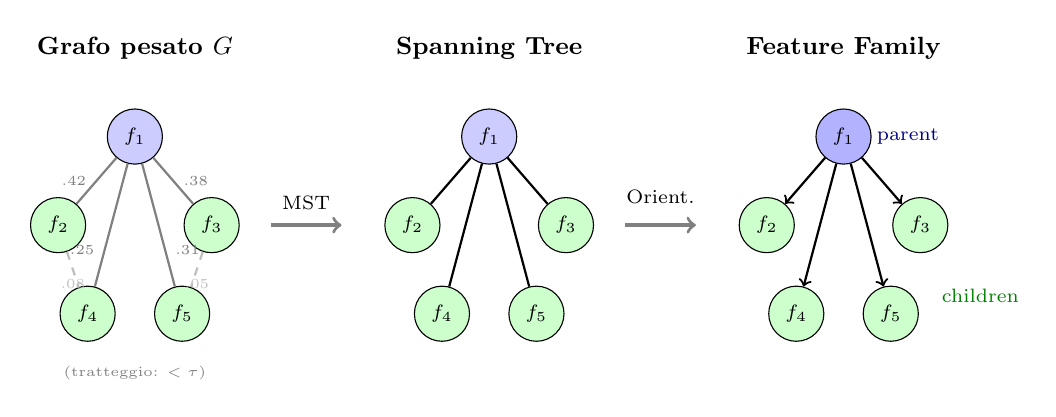
\begin{tikzpicture}[scale=0.75]
        
        % === PASSO 1-2: Grafo pesato ===
        \node[font=\small\bfseries] at (0, 3.5) {Grafo pesato $G$};
        
        \node[draw, circle, fill=blue!20, minimum size=0.7cm, font=\scriptsize] (A) at (0, 2) {$f_1$};
        \node[draw, circle, fill=green!20, minimum size=0.7cm, font=\scriptsize] (B) at (-1.3, 0.5) {$f_2$};
        \node[draw, circle, fill=green!20, minimum size=0.7cm, font=\scriptsize] (C) at (1.3, 0.5) {$f_3$};
        \node[draw, circle, fill=green!20, minimum size=0.7cm, font=\scriptsize] (D) at (-0.8, -1) {$f_4$};
        \node[draw, circle, fill=green!20, minimum size=0.7cm, font=\scriptsize] (E) at (0.8, -1) {$f_5$};
        
        \draw[thick, gray] (A) -- node[left, font=\tiny] {.42} (B);
        \draw[thick, gray] (A) -- node[right, font=\tiny] {.38} (C);
        \draw[thick, gray] (A) -- node[left, font=\tiny, pos=0.7] {.25} (D);
        \draw[thick, gray] (A) -- node[right, font=\tiny, pos=0.7] {.31} (E);
        \draw[thick, gray!50, dashed] (B) -- node[below, font=\tiny] {.08} (D);
        \draw[thick, gray!50, dashed] (C) -- node[below, font=\tiny] {.05} (E);
        
        \node[font=\tiny, gray] at (0, -2) {(tratteggio: $< \tau$)};
        
        % Freccia
        \draw[->, very thick, gray] (2.3, 0.5) -- (3.5, 0.5);
        \node[above, font=\scriptsize] at (2.9, 0.6) {MST};
        
        % === PASSO 3: MST ===
        \begin{scope}[shift={(6, 0)}]
            \node[font=\small\bfseries] at (0, 3.5) {Spanning Tree};
            
            \node[draw, circle, fill=blue!20, minimum size=0.7cm, font=\scriptsize] (A2) at (0, 2) {$f_1$};
            \node[draw, circle, fill=green!20, minimum size=0.7cm, font=\scriptsize] (B2) at (-1.3, 0.5) {$f_2$};
            \node[draw, circle, fill=green!20, minimum size=0.7cm, font=\scriptsize] (C2) at (1.3, 0.5) {$f_3$};
            \node[draw, circle, fill=green!20, minimum size=0.7cm, font=\scriptsize] (D2) at (-0.8, -1) {$f_4$};
            \node[draw, circle, fill=green!20, minimum size=0.7cm, font=\scriptsize] (E2) at (0.8, -1) {$f_5$};
            
            \draw[thick] (A2) -- (B2);
            \draw[thick] (A2) -- (C2);
            \draw[thick] (A2) -- (D2);
            \draw[thick] (A2) -- (E2);
        \end{scope}
        
        % Freccia
        \draw[->, very thick, gray] (8.3, 0.5) -- (9.5, 0.5);
        \node[above, font=\scriptsize, align=center] at (8.9, 0.7) {Orient.};
        
        % === PASSO 4: DAG orientato ===
        \begin{scope}[shift={(12, 0)}]
            \node[font=\small\bfseries] at (0, 3.5) {Feature Family};
            
            \node[draw, circle, fill=blue!30, minimum size=0.7cm, font=\scriptsize] (A3) at (0, 2) {$f_1$};
            \node[draw, circle, fill=green!20, minimum size=0.7cm, font=\scriptsize] (B3) at (-1.3, 0.5) {$f_2$};
            \node[draw, circle, fill=green!20, minimum size=0.7cm, font=\scriptsize] (C3) at (1.3, 0.5) {$f_3$};
            \node[draw, circle, fill=green!20, minimum size=0.7cm, font=\scriptsize] (D3) at (-0.8, -1) {$f_4$};
            \node[draw, circle, fill=green!20, minimum size=0.7cm, font=\scriptsize] (E3) at (0.8, -1) {$f_5$};
            
            \draw[->, thick] (A3) -- (B3);
            \draw[->, thick] (A3) -- (C3);
            \draw[->, thick] (A3) -- (D3);
            \draw[->, thick] (A3) -- (E3);
            
            \node[right, font=\scriptsize, blue!50!black] at (0.4, 2) {parent};
            \node[right, font=\scriptsize, green!50!black] at (1.5, -0.7) {children};
        \end{scope}
        
    \end{tikzpicture}
    \caption{Costruzione di una feature family. (Sinistra) Il grafo pesato $G$ con pesi $C^{\text{norm}}_{ij}$; gli archi tratteggiati sono sotto soglia e verranno rimossi. (Centro) Il Maximum Spanning Tree preserva solo le connessioni più forti. (Destra) L'orientamento basato sulla frequenza $f_i$ rivela la struttura gerarchica: $f_1$ (parent) punta verso i children meno frequenti.}
    \label{fig:family_construction}
\end{figure}
Nel grafo orientato risultante, le \textbf{radici}---nodi senza archi entranti---sono i parent delle famiglie. A partire da ciascuna radice, una visita in profondità (depth-first search) raccoglie tutti i discendenti, formando una feature family. La struttura tipica è a stella: il parent è connesso direttamente a tutti i children, che raramente sono connessi tra loro. Questa topologia riflette la struttura gerarchica dei concetti: il parent cattura un tema generale, i children catturano sotto-temi specifici che condividono il tema generale ma non si sovrappongono tra loro.
Le feature families catturano la struttura gerarchica naturale dei concetti in un dominio. Nel dataset di O'Neill et al.\ su paper di machine learning, emergono famiglie come \textit{Optimization Techniques} (parent) con children \textit{Gradient Descent}, \textit{Adam}, \textit{RMSprop}, \textit{Momentum}; oppure \textit{Transformer models} (parent) con children \textit{Vision Transformers}, \textit{Positional Encoding}, \textit{Attention mechanisms}. Nel contesto medico-pediatrico di PRISMA, ci aspettiamo famiglie analoghe, come \textit{Infezioni respiratorie} (parent) con children \textit{Polmonite}, \textit{Bronchiolite}, \textit{Faringite}.

% [NOTA: Qui inserirò screenshot di PRISMA che mostra il grafo di una feature family]
Le feature families non sono solo un artefatto dell'analisi: riflettono come il SAE ha imparato a organizzare i concetti del dominio, e forniscono una mappa navigabile della conoscenza codificata nelle rappresentazioni sparse.

\subsubsection{Feature splitting: evoluzione inter-SAE}
\label{subsubsec:feature_splitting}

Le feature families descrivono la struttura \textit{all'interno} di un singolo SAE. Ma cosa succede quando confrontiamo SAE di capacità diverse addestrati sugli stessi dati? Emergono tre fenomeni distinti: alcune feature riappaiono identiche (\textit{feature ricorrenti}), altre si scindono in sotto-concetti più specifici (\textit{feature splitting}), altre ancora compaiono per la prima volta (\textit{feature nuove}).

Per studiare questi fenomeni, O'Neill et al.~\parencite{oneill2024disentangling} confrontano SAE con diversi valori di $k$ (numero di feature attive per documento) e $n$ (dimensione dello spazio latente), utilizzando due metriche complementari che catturano aspetti diversi della relazione tra feature.

La \textbf{similarità geometrica} $S_{ij}$, definita in Sezione~\ref{subsubsec:notation_matrices}, confronta le \textit{direzioni} dei vettori decoder $\mathbf{w}_i$ e $\mathbf{w}_j$ nello spazio degli embedding. È una proprietà dei pesi appresi: risponde alla domanda ``queste due feature puntano nella stessa direzione semantica?''. Può essere calcolata anche senza passare alcun documento attraverso il SAE.

La \textbf{similarità di attivazione} confronta invece i \textit{pattern di attivazione} sui documenti. Ogni feature $i$ ha un profilo di attivazione sull'intero corpus, rappresentato dalla colonna $i$-esima della matrice $H$. Due feature con alta similarità di attivazione si ``accendono'' sugli stessi documenti, con intensità correlate. È una proprietà del comportamento sui dati: risponde alla domanda ``queste due feature reagiscono agli stessi input?''.

\begin{table}[htbp]
    \centering
    \caption{Confronto tra le due metriche per l'analisi delle feature.}
    \label{tab:similarity_comparison}
    \begin{tabular}{@{}p{2.8cm}p{4.5cm}p{4.5cm}@{}}
        \toprule
        & \textbf{Similarità geometrica} $S$ & \textbf{Similarità di attivazione} $D$ \\
        \midrule
        Cosa confronta & Direzioni nello spazio embedding & Pattern di attivazione sui documenti \\[0.5em]
        Vettori coinvolti & $\mathbf{w}_i, \mathbf{w}_j \in \mathbb{R}^d$ & Colonne di $H \in \mathbb{R}^N$ \\[0.5em]
        Dipende dai dati? & No (solo pesi del decoder) & Sì (richiede il corpus) \\[0.5em]
        Domanda chiave & ``Dove puntano?'' & ``Quando si accendono?'' \\
        \bottomrule
    \end{tabular}
\end{table}

La similarità geometrica ha un'interpretazione immediata in termini di angoli. Poiché $S_{ij}$ è definita come il coseno tra i vettori decoder, vale:
\begin{equation}
    S_{ij} = \cos(\theta_{ij})
    \label{eq:similarity_angle}
\end{equation}
dove $\theta_{ij}$ è l'angolo tra le direzioni $\mathbf{w}_i$ e $\mathbf{w}_j$ nello spazio degli embedding. Le soglie di similarità corrispondono quindi a soglie angolari: $S = 0.95$ equivale a $\theta \approx 18°$ (direzioni quasi parallele), $S = 0.5$ equivale a $\theta = 60°$ (angolo moderato), $S = 0$ equivale a $\theta = 90°$ (direzioni ortogonali).

Perché servono entrambe le metriche? Consideriamo i casi limite. Due feature potrebbero puntare in direzioni simili ($S$ alta) ma attivarsi su documenti completamente diversi ($D$ bassa)---un caso raro, possibile artefatto del training. Viceversa, due feature potrebbero rappresentare concetti semanticamente distinti ($S$ bassa) ma co-occorrere frequentemente ($D$ alta)---ad esempio ``febbre'' e ``infezione'', concetti diversi che compaiono spesso insieme.

Data una coppia di SAE---uno ``piccolo'' con $n_1$ feature e uno ``grande'' con $n_2$ feature ($n_1 < n_2$)---per ogni feature $j$ del SAE grande si identifica il \textbf{nearest neighbour} nel SAE piccolo:
\begin{equation}
    i^*(j) = \underset{i \in \{1,\dots,n_1\}}{\mathrm{arg\,max}} \; S_{ij}
    \label{eq:nearest_neighbour}
\end{equation}
e si calcola sia la similarità geometrica massima $S^*_j = S_{i^*(j), j}$, sia la similarità di attivazione tra $j$ e $i^*(j)$. Combinando le due metriche, ogni feature del SAE grande può essere classificata:

\begin{enumerate}
    \item \textbf{Feature ricorrenti.} Caratterizzate da alta similarità geometrica ($S^*_j > 0.95$, ovvero $\theta < 18°$) \textit{e} alta similarità di attivazione. Riappaiono sostanzialmente invariate nel SAE più grande. Rappresentano concetti ``atomici'' che non si scompongono ulteriormente all'aumentare della capacità---ad esempio, ``O-type stars'' in astrofisica o ``Generative Adversarial Networks'' in machine learning.
    
    \item \textbf{Feature da splitting.} Caratterizzate da similarità geometrica moderata ($0.5 < S^*_j < 0.95$, ovvero $18° < \theta < 60°$) e similarità di attivazione parziale. Emergono dalla scissione di una feature più generale: si attivano su un \textit{sottoinsieme} dei documenti che attivavano la feature parent. Ad esempio, ``Periodicity detection'' nel SAE piccolo potrebbe scindersi in ``Quasi-periodic oscillations in blazars'' e ``Pulsar timing'' nel SAE grande.
    
    \item \textbf{Feature nuove.} Caratterizzate da bassa similarità geometrica ($S^*_j < 0.5$, ovvero $\theta > 60°$) \textit{oppure} bassa similarità di attivazione. Non hanno corrispondenti nel SAE più piccolo: il concetto non era rappresentabile con la capacità precedente.
\end{enumerate}

\begin{figure}[htbp]
    \centering
    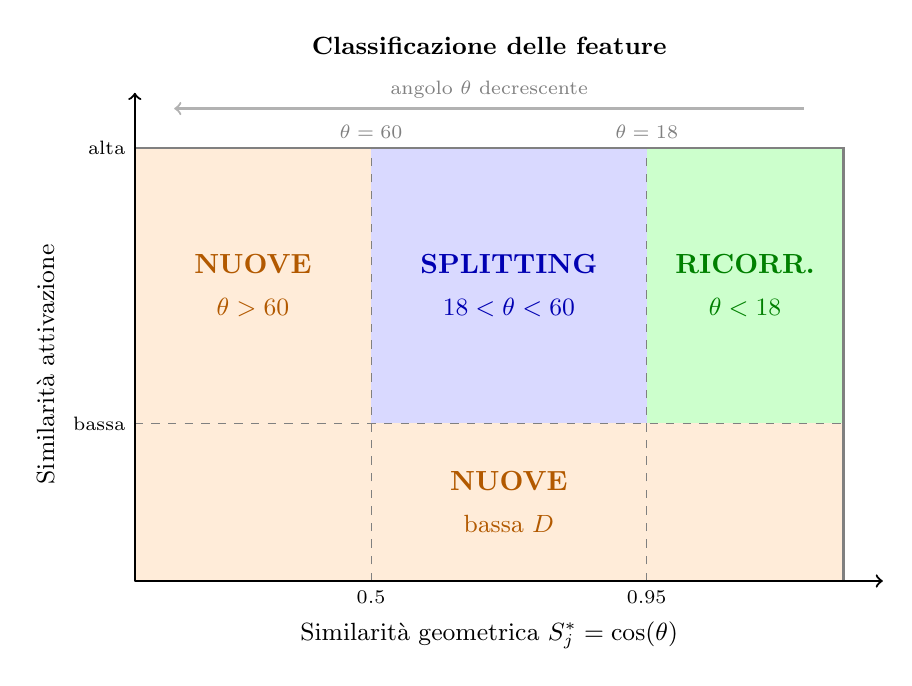
\begin{tikzpicture}[scale=1.0]
        
        % Titolo
        \node[font=\small\bfseries] at (4.5, 6.8) {Classificazione delle feature};
        
        % Griglia di sfondo
        \fill[orange!15] (0, 0) rectangle (9, 5.5);
        \fill[blue!15] (3, 2) rectangle (6.5, 5.5);
        \fill[green!20] (6.5, 2) rectangle (9, 5.5);
        
        % Bordi regioni
        \draw[thick, gray] (0, 0) rectangle (9, 5.5);
        \draw[dashed, gray] (3, 0) -- (3, 5.5);
        \draw[dashed, gray] (6.5, 0) -- (6.5, 5.5);
        \draw[dashed, gray] (0, 2) -- (9, 2);
        
        % Assi
        \draw[->, thick] (0, 0) -- (9.5, 0);
        \draw[->, thick] (0, 0) -- (0, 6.2);
        
        % Labels assi
        \node[below, font=\small] at (4.5, -0.4) {Similarità geometrica $S^*_j = \cos(\theta)$};
        \node[left, font=\small, rotate=90, anchor=south] at (-0.9, 2.75) {Similarità attivazione};
        
        % Labels soglie similarità
        \node[below, font=\scriptsize] at (3, 0) {$0.5$};
        \node[below, font=\scriptsize] at (6.5, 0) {$0.95$};
        \node[left, font=\scriptsize] at (0, 2) {bassa};
        \node[left, font=\scriptsize] at (0, 5.5) {alta};
        
        % Labels soglie angolari (sopra)
        \node[above, font=\scriptsize, gray] at (3, 5.5) {$\theta = 60°$};
        \node[above, font=\scriptsize, gray] at (6.5, 5.5) {$\theta = 18°$};
        
        % Freccia direzione angolo
        \draw[<-, thick, gray!60] (0.5, 6.0) -- (8.5, 6.0);
        \node[above, font=\scriptsize, gray] at (4.5, 6.0) {angolo $\theta$ decrescente};
        
        % Labels regioni
        \node[font=\normalsize, orange!70!black, align=center] at (1.5, 3.75) {\textbf{NUOVE}\\[0.3em]\small $\theta > 60°$};
        \node[font=\normalsize, orange!70!black, align=center] at (4.75, 1) {\textbf{NUOVE}\\[0.3em]\small bassa $D$};
        \node[font=\normalsize, blue!70!black, align=center] at (4.75, 3.75) {\textbf{SPLITTING}\\[0.3em]\small $18° < \theta < 60°$};
        \node[font=\normalsize, green!50!black, align=center] at (7.75, 3.75) {\textbf{RICORR.}\\[0.3em]\small $\theta < 18°$};
        
    \end{tikzpicture}
    \caption{Classificazione delle feature del SAE grande rispetto al SAE piccolo. L'asse orizzontale misura la similarità geometrica $S^*_j = \cos(\theta)$, dove $\theta$ è l'angolo tra i vettori decoder. Le soglie di similarità corrispondono a soglie angolari: feature \textbf{ricorrenti} hanno direzioni quasi parallele ($\theta < 18°$), feature da \textbf{splitting} formano angoli moderati ($18°$--$60°$), feature \textbf{nuove} puntano in direzioni molto diverse ($\theta > 60°$) oppure hanno bassa similarità di attivazione.}
    \label{fig:feature_classification}
\end{figure}

Lo splitting può essere compreso anche geometricamente. Se una feature $\mathbf{w}_p$ del SAE piccolo rappresenta un concetto generale, nel SAE grande questo concetto può scindersi in $m$ feature $\mathbf{w}_{c_1}, \dots, \mathbf{w}_{c_m}$ che rappresentano sotto-concetti. La direzione del parent è approssimativamente una combinazione delle direzioni dei children:
\begin{equation}
    \mathbf{w}_p \approx \sum_{i=1}^{m} \alpha_i \, \mathbf{w}_{c_i}
    \label{eq:splitting_geometry}
\end{equation}
dove i coefficienti $\alpha_i$ riflettono il ``peso'' relativo di ogni sotto-concetto. Ogni child ha similarità moderata con il parent (angolo $18°$--$60°$) ma bassa similarità con gli altri children (angolo $> 60°$), riflettendo la specializzazione semantica.

\begin{figure}[htbp]
    \centering
    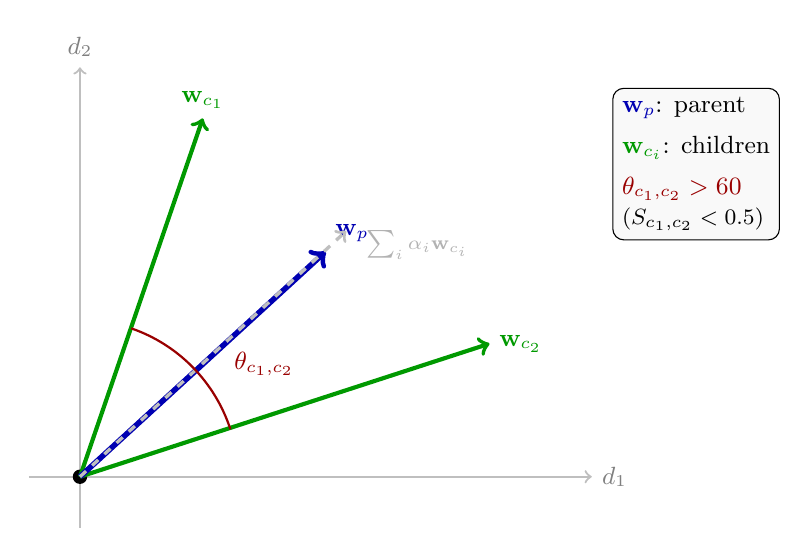
\begin{tikzpicture}[scale=1.3]
        
        % Assi
        \draw[->, thick, gray!50] (-0.5, 0) -- (5, 0) node[right, font=\small, gray] {$d_1$};
        \draw[->, thick, gray!50] (0, -0.5) -- (0, 4) node[above, font=\small, gray] {$d_2$};
        
        % Origine
        \coordinate (O) at (0, 0);
        \fill (O) circle (2pt);
        
        % Child 1 (più verticale)
        \coordinate (Wc1) at (1.2, 3.5);
        \draw[->, thick, green!60!black, line width=1.5pt] (O) -- (Wc1);
        \node[above, font=\small, green!60!black] at (Wc1) {$\mathbf{w}_{c_1}$};
        
        % Child 2 (più orizzontale)
        \coordinate (Wc2) at (4, 1.3);
        \draw[->, thick, green!60!black, line width=1.5pt] (O) -- (Wc2);
        \node[right, font=\small, green!60!black] at (Wc2) {$\mathbf{w}_{c_2}$};
        
        % Parent (nel mezzo)
        \coordinate (Wp) at (2.4, 2.2);
        \draw[->, very thick, blue!70!black, line width=2pt] (O) -- (Wp);
        \node[above right, font=\small, blue!70!black] at (Wp) {$\mathbf{w}_p$};
        
        % Somma pesata (tratteggiato, vicino al parent)
        \coordinate (Sum) at (2.6, 2.4);
        \draw[->, thick, gray!50, dashed, line width=1.2pt] (O) -- (Sum);
        \node[below right, font=\scriptsize, gray!60] at (2.7, 2.5) {$\sum_i \alpha_i \mathbf{w}_{c_i}$};
        
        % Arco angolo grande tra children
        \draw[thick, red!60!black] (0.5, 1.45) arc[start angle=71, end angle=18, radius=1.55];
        \node[font=\small, red!60!black] at (1.8, 1.1) {$\theta_{c_1, c_2}$};
        
        % Box legenda
        \node[draw, rectangle, rounded corners, fill=gray!5, font=\small, align=left, anchor=north west] at (5.2, 3.8) {
            \textcolor{blue!70!black}{$\mathbf{w}_p$}: parent\\[0.4em]
            \textcolor{green!60!black}{$\mathbf{w}_{c_i}$}: children\\[0.4em]
            \textcolor{red!60!black}{$\theta_{c_1,c_2} > 60°$}\\
            \footnotesize$(S_{c_1,c_2} < 0.5)$
        };
        
    \end{tikzpicture}
    \caption{Interpretazione geometrica del feature splitting. I children $\mathbf{w}_{c_1}$ e $\mathbf{w}_{c_2}$ (verde) rappresentano sotto-concetti specializzati nel SAE grande. Il parent $\mathbf{w}_p$ (blu) del SAE piccolo punta nella direzione della loro combinazione pesata. L'angolo $\theta_{c_1,c_2} > 60°$ tra i children corrisponde a similarità $S < 0.5$: i sotto-concetti sono semanticamente distinti tra loro.}
    \label{fig:splitting_geometry}
\end{figure}

\begin{figure}[htbp]
    \centering
    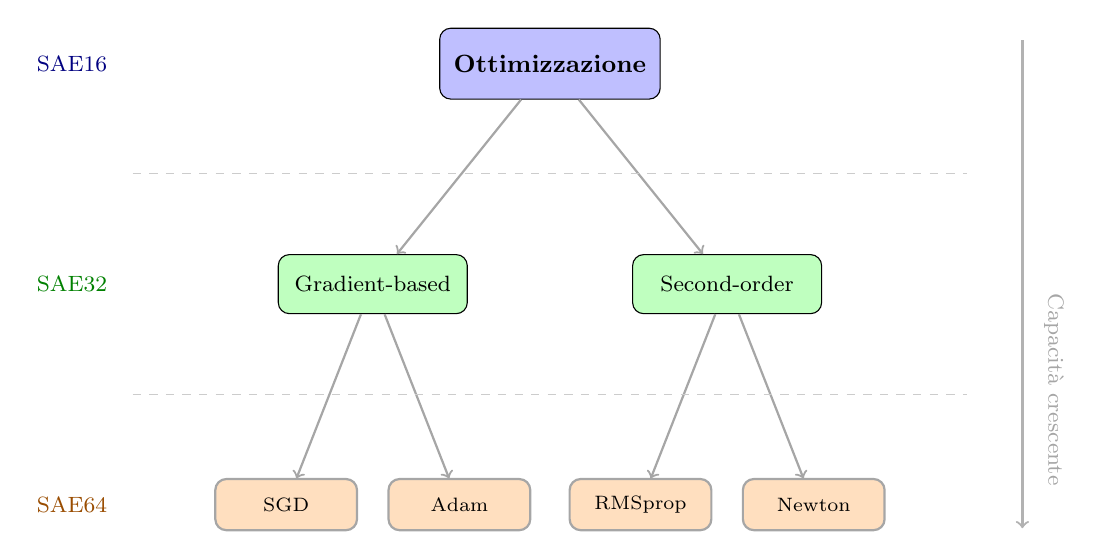
\begin{tikzpicture}[
        level 1/.style={sibling distance=4.5cm, level distance=2.8cm},
        level 2/.style={sibling distance=2.2cm, level distance=2.8cm},
        every node/.style={font=\small},
        edge from parent/.style={draw, ->, thick, gray!70},
        sae16/.style={draw, rectangle, rounded corners, fill=blue!25, minimum width=2.8cm, minimum height=0.9cm, font=\small\bfseries},
        sae32/.style={draw, rectangle, rounded corners, fill=green!25, minimum width=2.4cm, minimum height=0.75cm, font=\footnotesize},
        sae64/.style={draw, rectangle, rounded corners, fill=orange!25, minimum width=1.8cm, minimum height=0.65cm, font=\scriptsize}
    ]
        
        % Albero
        \node[sae16] {Ottimizzazione}
            child {
                node[sae32] {Gradient-based}
                child {node[sae64] {SGD}}
                child {node[sae64] {Adam}}
            }
            child {
                node[sae32] {Second-order}
                child {node[sae64] {RMSprop}}
                child {node[sae64] {Newton}}
            };
        
        % Etichette dei livelli (a sinistra)
        \node[left, font=\footnotesize, blue!50!black] at (-5.5, 0) {SAE16};
        \node[left, font=\footnotesize, green!50!black] at (-5.5, -2.8) {SAE32};
        \node[left, font=\footnotesize, orange!60!black] at (-5.5, -5.6) {SAE64};
        
        % Linee tratteggiate orizzontali per i livelli
        \draw[dashed, gray!40] (-5.3, -1.4) -- (5.3, -1.4);
        \draw[dashed, gray!40] (-5.3, -4.2) -- (5.3, -4.2);
        
        % Freccia capacità crescente (a destra)
        \draw[->, thick, gray!60] (6, 0.3) -- (6, -5.9);
        \node[right, font=\footnotesize, gray!70, align=left, rotate=-90] at (6.4, -2.8) {Capacità crescente};
        
    \end{tikzpicture}
    \caption{Il fenomeno del \emph{feature splitting}. Una feature generale (``Ottimizzazione'') appresa da un SAE a bassa capacità (SAE16) si scinde progressivamente in feature più specifiche quando la capacità aumenta. SAE32 distingue metodi gradient-based da metodi del secondo ordine; SAE64 risolve i singoli algoritmi. La struttura ad albero emerge spontaneamente dall'analisi delle similarità tra feature di modelli diversi.}
    \label{fig:feature_splitting}
\end{figure}

Il fenomeno dello splitting ha implicazioni pratiche importanti: SAE più grandi non apprendono semplicemente ``più feature'', ma apprendono feature \textit{più specifiche}. La capacità del SAE determina il livello di granularità concettuale raggiungibile: un SAE piccolo cattura solo i macro-concetti, un SAE grande distingue sfumature più sottili. La scelta della capacità diventa quindi un trade-off tra interpretabilità (poche feature generali, facili da etichettare) e precisione semantica (molte feature specifiche, più informative).

% [NOTA: Qui inserirò screenshot di PRISMA che mostra il confronto tra SAE di capacità diverse]


%%%%%%%%%%%%%%%%%%%%%%%%%%%%%%%%%%%%%%%%%%%%%%%%%%%%%%%%
\subsubsection{Quantificare la struttura: Effective Rank}
\label{subsubsec:effective_rank}


Questa sezione presenta un contributo originale di questa tesi: l'applicazione dell'Effective Rank alla matrice di attivazione degli Sparse Autoencoder come metrica per quantificare la compressione semantica.
Le sezioni precedenti hanno mostrato che le feature apprese da un SAE non sono indipendenti: si organizzano in famiglie gerarchiche (Sezione~\ref{subsubsec:feature_families}) e si scindono progressivamente al crescere della capacità (Sezione~\ref{subsubsec:feature_splitting}). Queste strutture implicano \textit{correlazioni sistematiche} nella matrice di attivazione $H$: feature della stessa famiglia tendono a co-attivarsi, feature da splitting si attivano su sottoinsiemi sovrapposti di documenti.
Una conseguenza diretta è che la matrice $H \in \mathbb{R}^{N \times n}$, pur avendo $n$ colonne (feature), non utilizza realmente $n$ gradi di libertà indipendenti. La dimensionalità \textit{effettiva} del codice sparso è inferiore alla dimensionalità nominale. Quantificare questo gap permette di misurare quanto la struttura semantica del dominio ``comprime'' le rappresentazioni apprese.
Il rango matriciale classico non è adatto a questo scopo: è instabile in presenza di rumore e restituisce un intero, perdendo informazione sulla distribuzione della varianza tra le direzioni. Per questo adottiamo l'\textbf{Effective Rank}~\parencite{roy2007effective}, una misura continua e robusta della dimensionalità intrinseca basata sull'entropia dello spettro singolare.
Sia $H = U \Sigma V^T$ la decomposizione ai valori singolari (SVD) della matrice di attivazione, con valori singolari $\sigma_1 \geq \sigma_2 \geq \dots \geq \sigma_Q \geq 0$, dove $Q = \min(N, n)$. Si definisce la \textbf{distribuzione normalizzata} dei valori singolari:
\begin{equation}
    p_i = \frac{\sigma_i}{\sum_{j=1}^{Q} \sigma_j} = \frac{\sigma_i}{\|\boldsymbol{\sigma}\|_1}
    \label{eq:singular_distribution}
\end{equation}
dove $\|\boldsymbol{\sigma}\|_1$ è la norma $\ell_1$ del vettore dei valori singolari. La distribuzione $\{p_i\}$ soddisfa $p_i \geq 0$ e $\sum_i p_i = 1$, e può essere interpretata come una distribuzione di probabilità che descrive come la ``varianza'' totale della matrice è distribuita tra le diverse direzioni singolari.
L'\textbf{Effective Rank} è definito come l'esponenziale dell'entropia di Shannon di questa distribuzione:
\begin{equation}
    \text{ER}(H) = \exp\left( -\sum_{i=1}^{Q} p_i \log p_i \right) = \exp\bigl( H(\mathbf{p}) \bigr)
    \label{eq:effective_rank}
\end{equation}
dove $H(\mathbf{p})$ è l'entropia della distribuzione $\{p_i\}$, con la convenzione $0 \log 0 = 0$.
L'effective rank ha un'interpretazione intuitiva legata alla distribuzione della varianza:
\begin{itemize}
    \item Se tutti i valori singolari sono uguali ($\sigma_i = \sigma$ per ogni $i$), allora $p_i = 1/Q$ per ogni $i$, l'entropia è massima ($H = \log Q$), e $\text{ER}(H) = Q$: la matrice utilizza tutte le direzioni in modo uniforme.    
    \item Se un solo valore singolare domina ($\sigma_1 \gg \sigma_{i>1}$), allora $p_1 \approx 1$ e $p_{i>1} \approx 0$, l'entropia è minima ($H \approx 0$), e $\text{ER}(H) \approx 1$: la matrice è essenzialmente unidimensionale.  
    \item Nei casi intermedi, $\text{ER}(H)$ restituisce un valore continuo che rappresenta il ``numero effettivo'' di direzioni indipendenti utilizzate dalla matrice.
\end{itemize}

\begin{figure}[htbp]
    \centering
    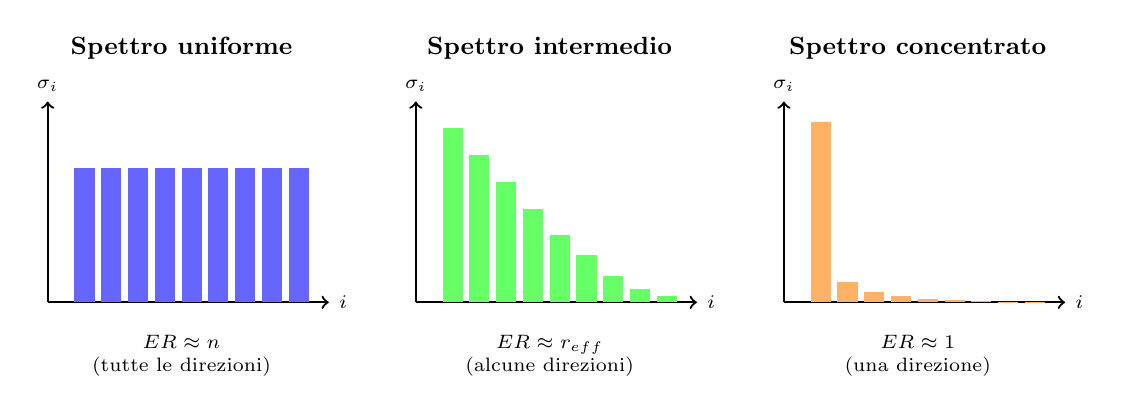
\begin{tikzpicture}[scale=0.85]
        
        % Caso 1: uniforme
        \begin{scope}[shift={(0, 0)}]
            \node[font=\small\bfseries] at (2, 3.8) {Spettro uniforme};
            \draw[->, thick] (0, 0) -- (4.2, 0) node[right, font=\scriptsize] {$i$};
            \draw[->, thick] (0, 0) -- (0, 3) node[above, font=\scriptsize] {$\sigma_i$};
            
            \foreach \x in {0.4, 0.8, 1.2, 1.6, 2.0, 2.4, 2.8, 3.2, 3.6} {
                \fill[blue!60] (\x, 0) rectangle (\x+0.3, 2);
            }
            
            \node[font=\scriptsize, align=center] at (2, -0.8) {$\text{ER} \approx n$\\(tutte le direzioni)};
        \end{scope}
        
        % Caso 2: decadimento graduale
        \begin{scope}[shift={(5.5, 0)}]
            \node[font=\small\bfseries] at (2, 3.8) {Spettro intermedio};
            \draw[->, thick] (0, 0) -- (4.2, 0) node[right, font=\scriptsize] {$i$};
            \draw[->, thick] (0, 0) -- (0, 3) node[above, font=\scriptsize] {$\sigma_i$};
            
            \fill[green!60] (0.4, 0) rectangle (0.7, 2.6);
            \fill[green!60] (0.8, 0) rectangle (1.1, 2.2);
            \fill[green!60] (1.2, 0) rectangle (1.5, 1.8);
            \fill[green!60] (1.6, 0) rectangle (1.9, 1.4);
            \fill[green!60] (2.0, 0) rectangle (2.3, 1.0);
            \fill[green!60] (2.4, 0) rectangle (2.7, 0.7);
            \fill[green!60] (2.8, 0) rectangle (3.1, 0.4);
            \fill[green!60] (3.2, 0) rectangle (3.5, 0.2);
            \fill[green!60] (3.6, 0) rectangle (3.9, 0.1);
            
            \node[font=\scriptsize, align=center] at (2, -0.8) {$\text{ER} \approx r_{\text{eff}}$\\(alcune direzioni)};
        \end{scope}
        
        % Caso 3: dominato
        \begin{scope}[shift={(11, 0)}]
            \node[font=\small\bfseries] at (2, 3.8) {Spettro concentrato};
            \draw[->, thick] (0, 0) -- (4.2, 0) node[right, font=\scriptsize] {$i$};
            \draw[->, thick] (0, 0) -- (0, 3) node[above, font=\scriptsize] {$\sigma_i$};
            
            \fill[orange!60] (0.4, 0) rectangle (0.7, 2.7);
            \fill[orange!60] (0.8, 0) rectangle (1.1, 0.3);
            \fill[orange!60] (1.2, 0) rectangle (1.5, 0.15);
            \fill[orange!60] (1.6, 0) rectangle (1.9, 0.1);
            \fill[orange!60] (2.0, 0) rectangle (2.3, 0.05);
            \fill[orange!60] (2.4, 0) rectangle (2.7, 0.03);
            \fill[orange!60] (2.8, 0) rectangle (3.1, 0.02);
            \fill[orange!60] (3.2, 0) rectangle (3.5, 0.01);
            \fill[orange!60] (3.6, 0) rectangle (3.9, 0.01);
            
            \node[font=\scriptsize, align=center] at (2, -0.8) {$\text{ER} \approx 1$\\(una direzione)};
        \end{scope}
        
    \end{tikzpicture}
    \caption{Interpretazione geometrica dell'Effective Rank. Lo spettro dei valori singolari $\{\sigma_i\}$ determina quante direzioni la matrice utilizza effettivamente. Uno spettro uniforme (sinistra) indica che tutte le direzioni contribuiscono equamente: $\text{ER} \approx n$. Uno spettro concentrato (destra) indica che una sola direzione domina: $\text{ER} \approx 1$. I casi reali (centro) mostrano un decadimento graduale, con $\text{ER}$ che quantifica il numero effettivo di direzioni informative.}
    \label{fig:effective_rank_spectrum}
\end{figure}
Nel contesto degli Sparse Autoencoder, l'effective rank della matrice di attivazione $H$ misura quante feature ``indipendenti'' il SAE sta effettivamente utilizzando. Se le feature fossero perfettamente scorrelate, ci aspetteremmo $\text{ER}(H) \approx n$. Ma la presenza di feature families e splitting introduce correlazioni che riducono l'effective rank: $\text{ER}(H) < n$.
Per isolare il contributo della \textit{struttura semantica} dei dati dalla compressione intrinseca dell'architettura, confrontiamo l'effective rank su dati reali con un'\textbf{ipotesi nulla}: addestriamo lo stesso SAE su input casuali non strutturati (embedding generati uniformemente). Il SAE addestrato su rumore non può apprendere correlazioni semantiche, quindi il suo effective rank $\text{ER}_{\text{null}}$ riflette solo i vincoli architetturali (Top-K, dimensione latente).
Definiamo il \textbf{Semantic Compression Ratio} (SCR) come la riduzione percentuale dell'effective rank dovuta alla semantica:
\begin{equation}
    \text{SCR}(\%) = 100 \cdot \frac{\text{ER}_{\text{null}} - \text{ER}_{\text{real}}}{\text{ER}_{\text{null}}}
    \label{eq:scr}
\end{equation}

Un valore di $\text{SCR} = 40\%$ significa che il 40\% della compressione osservata è attribuibile alla struttura semantica del dominio---le co-attivazioni tra concetti correlati (febbre $\leftrightarrow$ infezione), le gerarchie concettuali (polmonite $\subset$ infezioni respiratorie), e le dipendenze implicite nel corpus.

\begin{figure}[htbp]
    \centering
    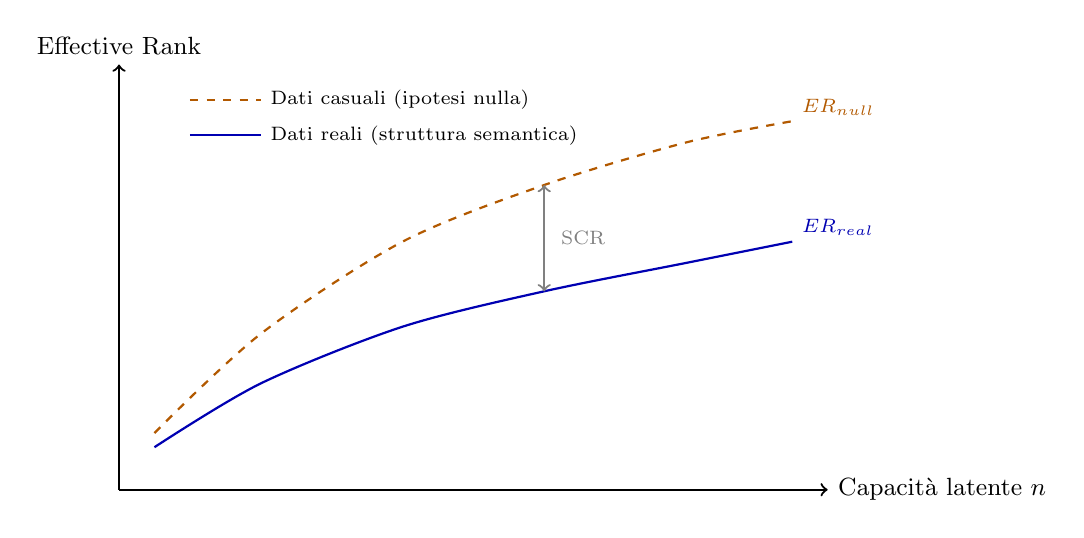
\begin{tikzpicture}[scale=0.9]
        
        % Assi
        \draw[->, thick] (0, 0) -- (10, 0) node[right, font=\small] {Capacità latente $n$};
        \draw[->, thick] (0, 0) -- (0, 6) node[above, font=\small] {Effective Rank};
        
        % Curva null (più alta)
        \draw[thick, orange!70!black, dashed] plot[smooth] coordinates {
            (0.5, 0.8) (2, 2.2) (4, 3.5) (6, 4.3) (8, 4.9) (9.5, 5.2)
        };
        \node[right, font=\scriptsize, orange!70!black] at (9.5, 5.4) {$\text{ER}_{\text{null}}$};
        
        % Curva real (più bassa)
        \draw[thick, blue!70!black] plot[smooth] coordinates {
            (0.5, 0.6) (2, 1.5) (4, 2.3) (6, 2.8) (8, 3.2) (9.5, 3.5)
        };
        \node[right, font=\scriptsize, blue!70!black] at (9.5, 3.7) {$\text{ER}_{\text{real}}$};
        
        % Gap annotato
        \draw[<->, thick, gray] (6, 2.8) -- (6, 4.3);
        \node[right, font=\scriptsize, gray, align=left] at (6.1, 3.55) {SCR};
        
        % Legenda
        \draw[thick, orange!70!black, dashed] (1, 5.5) -- (2, 5.5);
        \node[right, font=\scriptsize] at (2, 5.5) {Dati casuali (ipotesi nulla)};
        \draw[thick, blue!70!black] (1, 5) -- (2, 5);
        \node[right, font=\scriptsize] at (2, 5) {Dati reali (struttura semantica)};
        
    \end{tikzpicture}
    \caption{Andamento qualitativo dell'Effective Rank al variare della capacità del SAE. Su dati casuali (tratteggiato), l'ER cresce linearmente con $n$: non ci sono correlazioni da sfruttare. Su dati reali (linea continua), l'ER cresce più lentamente: la struttura semantica introduce correlazioni che riducono la dimensionalità effettiva. Il gap tra le due curve, quantificato dal Semantic Compression Ratio, misura la ``compressione semantica'' del dominio.}
    \label{fig:er_scaling}
\end{figure}
L'analisi dell'effective rank fornisce una prospettiva complementare alle feature families e allo splitting:
\begin{itemize}
    \item Le \textbf{feature families} descrivono la struttura \textit{locale}: quali feature sono correlate tra loro.
    \item Il \textbf{feature splitting} descrive l'evoluzione \textit{inter-modello}: come le feature si raffinano al crescere della capacità.
    \item L'\textbf{effective rank} fornisce una misura \textit{globale}: quanta ridondanza complessiva esiste nel codice sparso.
\end{itemize}
I risultati empirici dell'analisi dell'effective rank su PRISMA saranno presentati nel Capitolo~\ref{chap:results}.